% Options for packages loaded elsewhere
\PassOptionsToPackage{unicode}{hyperref}
\PassOptionsToPackage{hyphens}{url}
%
\documentclass[
]{book}
\usepackage{amsmath,amssymb}
\usepackage{iftex}
\ifPDFTeX
  \usepackage[T1]{fontenc}
  \usepackage[utf8]{inputenc}
  \usepackage{textcomp} % provide euro and other symbols
\else % if luatex or xetex
  \usepackage{unicode-math} % this also loads fontspec
  \defaultfontfeatures{Scale=MatchLowercase}
  \defaultfontfeatures[\rmfamily]{Ligatures=TeX,Scale=1}
\fi
\usepackage{lmodern}
\ifPDFTeX\else
  % xetex/luatex font selection
\fi
% Use upquote if available, for straight quotes in verbatim environments
\IfFileExists{upquote.sty}{\usepackage{upquote}}{}
\IfFileExists{microtype.sty}{% use microtype if available
  \usepackage[]{microtype}
  \UseMicrotypeSet[protrusion]{basicmath} % disable protrusion for tt fonts
}{}
\makeatletter
\@ifundefined{KOMAClassName}{% if non-KOMA class
  \IfFileExists{parskip.sty}{%
    \usepackage{parskip}
  }{% else
    \setlength{\parindent}{0pt}
    \setlength{\parskip}{6pt plus 2pt minus 1pt}}
}{% if KOMA class
  \KOMAoptions{parskip=half}}
\makeatother
\usepackage{xcolor}
\usepackage{color}
\usepackage{fancyvrb}
\newcommand{\VerbBar}{|}
\newcommand{\VERB}{\Verb[commandchars=\\\{\}]}
\DefineVerbatimEnvironment{Highlighting}{Verbatim}{commandchars=\\\{\}}
% Add ',fontsize=\small' for more characters per line
\usepackage{framed}
\definecolor{shadecolor}{RGB}{248,248,248}
\newenvironment{Shaded}{\begin{snugshade}}{\end{snugshade}}
\newcommand{\AlertTok}[1]{\textcolor[rgb]{0.94,0.16,0.16}{#1}}
\newcommand{\AnnotationTok}[1]{\textcolor[rgb]{0.56,0.35,0.01}{\textbf{\textit{#1}}}}
\newcommand{\AttributeTok}[1]{\textcolor[rgb]{0.13,0.29,0.53}{#1}}
\newcommand{\BaseNTok}[1]{\textcolor[rgb]{0.00,0.00,0.81}{#1}}
\newcommand{\BuiltInTok}[1]{#1}
\newcommand{\CharTok}[1]{\textcolor[rgb]{0.31,0.60,0.02}{#1}}
\newcommand{\CommentTok}[1]{\textcolor[rgb]{0.56,0.35,0.01}{\textit{#1}}}
\newcommand{\CommentVarTok}[1]{\textcolor[rgb]{0.56,0.35,0.01}{\textbf{\textit{#1}}}}
\newcommand{\ConstantTok}[1]{\textcolor[rgb]{0.56,0.35,0.01}{#1}}
\newcommand{\ControlFlowTok}[1]{\textcolor[rgb]{0.13,0.29,0.53}{\textbf{#1}}}
\newcommand{\DataTypeTok}[1]{\textcolor[rgb]{0.13,0.29,0.53}{#1}}
\newcommand{\DecValTok}[1]{\textcolor[rgb]{0.00,0.00,0.81}{#1}}
\newcommand{\DocumentationTok}[1]{\textcolor[rgb]{0.56,0.35,0.01}{\textbf{\textit{#1}}}}
\newcommand{\ErrorTok}[1]{\textcolor[rgb]{0.64,0.00,0.00}{\textbf{#1}}}
\newcommand{\ExtensionTok}[1]{#1}
\newcommand{\FloatTok}[1]{\textcolor[rgb]{0.00,0.00,0.81}{#1}}
\newcommand{\FunctionTok}[1]{\textcolor[rgb]{0.13,0.29,0.53}{\textbf{#1}}}
\newcommand{\ImportTok}[1]{#1}
\newcommand{\InformationTok}[1]{\textcolor[rgb]{0.56,0.35,0.01}{\textbf{\textit{#1}}}}
\newcommand{\KeywordTok}[1]{\textcolor[rgb]{0.13,0.29,0.53}{\textbf{#1}}}
\newcommand{\NormalTok}[1]{#1}
\newcommand{\OperatorTok}[1]{\textcolor[rgb]{0.81,0.36,0.00}{\textbf{#1}}}
\newcommand{\OtherTok}[1]{\textcolor[rgb]{0.56,0.35,0.01}{#1}}
\newcommand{\PreprocessorTok}[1]{\textcolor[rgb]{0.56,0.35,0.01}{\textit{#1}}}
\newcommand{\RegionMarkerTok}[1]{#1}
\newcommand{\SpecialCharTok}[1]{\textcolor[rgb]{0.81,0.36,0.00}{\textbf{#1}}}
\newcommand{\SpecialStringTok}[1]{\textcolor[rgb]{0.31,0.60,0.02}{#1}}
\newcommand{\StringTok}[1]{\textcolor[rgb]{0.31,0.60,0.02}{#1}}
\newcommand{\VariableTok}[1]{\textcolor[rgb]{0.00,0.00,0.00}{#1}}
\newcommand{\VerbatimStringTok}[1]{\textcolor[rgb]{0.31,0.60,0.02}{#1}}
\newcommand{\WarningTok}[1]{\textcolor[rgb]{0.56,0.35,0.01}{\textbf{\textit{#1}}}}
\usepackage{longtable,booktabs,array}
\usepackage{calc} % for calculating minipage widths
% Correct order of tables after \paragraph or \subparagraph
\usepackage{etoolbox}
\makeatletter
\patchcmd\longtable{\par}{\if@noskipsec\mbox{}\fi\par}{}{}
\makeatother
% Allow footnotes in longtable head/foot
\IfFileExists{footnotehyper.sty}{\usepackage{footnotehyper}}{\usepackage{footnote}}
\makesavenoteenv{longtable}
\usepackage{graphicx}
\makeatletter
\def\maxwidth{\ifdim\Gin@nat@width>\linewidth\linewidth\else\Gin@nat@width\fi}
\def\maxheight{\ifdim\Gin@nat@height>\textheight\textheight\else\Gin@nat@height\fi}
\makeatother
% Scale images if necessary, so that they will not overflow the page
% margins by default, and it is still possible to overwrite the defaults
% using explicit options in \includegraphics[width, height, ...]{}
\setkeys{Gin}{width=\maxwidth,height=\maxheight,keepaspectratio}
% Set default figure placement to htbp
\makeatletter
\def\fps@figure{htbp}
\makeatother
\setlength{\emergencystretch}{3em} % prevent overfull lines
\providecommand{\tightlist}{%
  \setlength{\itemsep}{0pt}\setlength{\parskip}{0pt}}
\setcounter{secnumdepth}{5}
\usepackage{booktabs}
\usepackage{amsthm}
\makeatletter
\def\thm@space@setup{%
  \thm@preskip=8pt plus 2pt minus 4pt
  \thm@postskip=\thm@preskip
}
\makeatother
\usepackage{booktabs}
\usepackage{longtable}
\usepackage{array}
\usepackage{multirow}
\usepackage{wrapfig}
\usepackage{float}
\usepackage{colortbl}
\usepackage{pdflscape}
\usepackage{tabu}
\usepackage{threeparttable}
\usepackage{threeparttablex}
\usepackage[normalem]{ulem}
\usepackage{makecell}
\usepackage{xcolor}
\ifLuaTeX
  \usepackage{selnolig}  % disable illegal ligatures
\fi
\usepackage[]{natbib}
\bibliographystyle{apalike}
\usepackage{bookmark}
\IfFileExists{xurl.sty}{\usepackage{xurl}}{} % add URL line breaks if available
\urlstyle{same}
\hypersetup{
  pdftitle={Final Project-Group 04},
  pdfauthor={Shakib-241001661,Shudeshna-241000261,Mithun-241002261,Pradipto-241002161,Mufrad-241001461,Shahriar Islam-241000461},
  hidelinks,
  pdfcreator={LaTeX via pandoc}}

\title{Final Project-Group 04}
\author{Shakib-241001661,Shudeshna-241000261,Mithun-241002261,Pradipto-241002161,Mufrad-241001461,Shahriar Islam-241000461}
\date{2024-06-29}

\begin{document}
\maketitle

{
\setcounter{tocdepth}{1}
\tableofcontents
}
\chapter*{Objective of the Project}\label{objective-of-the-project}
\addcontentsline{toc}{chapter}{Objective of the Project}

perform \textbf{Regression} \& \textbf{Time Series analysis} and \textbf{forecasting techniques} on \emph{Bitcoin} historical price. The experience can be replicated to forecast Stock price \& Currency price as well.

\begin{Shaded}
\begin{Highlighting}[]
\FunctionTok{install.packages}\NormalTok{(}\StringTok{"bookdown"}\NormalTok{)}
\CommentTok{\# or the development version}
\CommentTok{\# devtools::install\_github("rstudio/bookdown")}
\end{Highlighting}
\end{Shaded}

\section*{Dataset}\label{dataset}
\addcontentsline{toc}{section}{Dataset}

A dataset of \textbf{Bitcoin} (BTC) historical price against USD. This is a monthly average price dataset having prices from 01 January 2015 to 30 November 2023.

\section*{Applied Model}\label{applied-model}
\addcontentsline{toc}{section}{Applied Model}

\begin{enumerate}
\def\labelenumi{\arabic{enumi}.}
\tightlist
\item
  Linear regression model
\item
  Quadratic regression model
\item
  ARMIA model
\end{enumerate}

\chapter{Data Preprocessing/Cleaning}\label{intro}

\section*{Loading the Dataset}\label{loading-the-dataset}
\addcontentsline{toc}{section}{Loading the Dataset}

\begin{itemize}
\tightlist
\item
  Load the dataset from csv into a data frame named BitCoin.
\item
  Check the data types of the features.
\item
  Assign appropriate data type to features.
\item
  Check the structure of the data frame.
\item
  Check if there's any missing value. If yes, treat missing values through appropriate methodology.
\end{itemize}

\subsection*{Load the dataset from csv into a data frame named BitCoin.}\label{load-the-dataset-from-csv-into-a-data-frame-named-bitcoin.}
\addcontentsline{toc}{subsection}{Load the dataset from csv into a data frame named BitCoin.}

\begin{Shaded}
\begin{Highlighting}[]
\CommentTok{\#("tidyverse")}
\CommentTok{\#Load the dataset from csv into a data frame named BitCoin.}
\FunctionTok{library}\NormalTok{(tidyverse)}
\end{Highlighting}
\end{Shaded}

\begin{verbatim}
## -- Attaching core tidyverse packages ------------------------ tidyverse 2.0.0 --
## v dplyr     1.1.4     v readr     2.1.5
## v forcats   1.0.0     v stringr   1.5.1
## v ggplot2   3.5.1     v tibble    3.2.1
## v lubridate 1.9.3     v tidyr     1.3.1
## v purrr     1.0.2     
## -- Conflicts ------------------------------------------ tidyverse_conflicts() --
## x dplyr::filter() masks stats::filter()
## x dplyr::lag()    masks stats::lag()
## i Use the conflicted package (<http://conflicted.r-lib.org/>) to force all conflicts to become errors
\end{verbatim}

\begin{Shaded}
\begin{Highlighting}[]
\CommentTok{\#load csv from github(uploaded for Assignment\_02\_Group\_04)}
\NormalTok{bitcoin }\OtherTok{\textless{}{-}} \FunctionTok{read.csv}\NormalTok{(}\StringTok{"https://raw.githubusercontent.com/shakibed/Final\_Project\_Group\_04/main/BTC{-}Monthly.csv"}\NormalTok{, }\AttributeTok{stringsAsFactors =} \ConstantTok{FALSE}\NormalTok{)}
\FunctionTok{view}\NormalTok{(bitcoin)}
\end{Highlighting}
\end{Shaded}

\section*{Check the data types of the features.}\label{check-the-data-types-of-the-features.}
\addcontentsline{toc}{section}{Check the data types of the features.}

\begin{Shaded}
\begin{Highlighting}[]
\CommentTok{\#Check the data types of the features.}
\FunctionTok{glimpse}\NormalTok{(bitcoin)}
\end{Highlighting}
\end{Shaded}

\begin{verbatim}
## Rows: 107
## Columns: 2
## $ Date  <chr> "2015-01-01", "2015-02-01", "2015-03-01", "2015-04-01", "2015-05~
## $ Close <dbl> 217.464, 254.263, 244.224, 236.145, 230.190, 263.072, 284.650, 2~
\end{verbatim}

\emph{\textbf{Code explanation here}}

We checked the data types using glimpse(bitcoin) and found we have two columns in data set.
We need to convert the Date column from chr (character) type to Date type because our target is to work with a time series object or perform linear regression analysis.

\section*{Assign appropriate data type to features.}\label{assign-appropriate-data-type-to-features.}
\addcontentsline{toc}{section}{Assign appropriate data type to features.}

\begin{Shaded}
\begin{Highlighting}[]
\NormalTok{bitcoin}\SpecialCharTok{$}\NormalTok{Date }\OtherTok{\textless{}{-}} \FunctionTok{as.Date}\NormalTok{(bitcoin}\SpecialCharTok{$}\NormalTok{Date)}
\FunctionTok{glimpse}\NormalTok{(bitcoin)}
\end{Highlighting}
\end{Shaded}

\begin{verbatim}
## Rows: 107
## Columns: 2
## $ Date  <date> 2015-01-01, 2015-02-01, 2015-03-01, 2015-04-01, 2015-05-01, 201~
## $ Close <dbl> 217.464, 254.263, 244.224, 236.145, 230.190, 263.072, 284.650, 2~
\end{verbatim}

\emph{\textbf{Code explanation here}}

\begin{itemize}
\tightlist
\item
  This will allow us to properly utilize the Date column in time series analysis or linear regression models.
\end{itemize}

\section*{Check the structure of the data frame.}\label{check-the-structure-of-the-data-frame.}
\addcontentsline{toc}{section}{Check the structure of the data frame.}

\begin{Shaded}
\begin{Highlighting}[]
\CommentTok{\#Check the data types of the features.}
\FunctionTok{str}\NormalTok{(bitcoin)}
\end{Highlighting}
\end{Shaded}

\begin{verbatim}
## 'data.frame':    107 obs. of  2 variables:
##  $ Date : Date, format: "2015-01-01" "2015-02-01" ...
##  $ Close: num  217 254 244 236 230 ...
\end{verbatim}

\emph{\textbf{Code explanation here}}

\begin{itemize}
\tightlist
\item
  We checked the structure of the data frame using str(bitcoin) and found the following:
\item
  The Date column is already in the Date format, and the Close column is of type num (numeric).
\item
  Since the Date column is correctly formatted as a date, it is ready for time series analysis or linear regression models without any further modification.
\end{itemize}

\section*{Check if there's any missing value. If yes, treat missing values through appropriate methodology.}\label{check-if-theres-any-missing-value.-if-yes-treat-missing-values-through-appropriate-methodology.}
\addcontentsline{toc}{section}{Check if there's any missing value. If yes, treat missing values through appropriate methodology.}

\begin{Shaded}
\begin{Highlighting}[]
\CommentTok{\#Check if there’s any missing value. If yes, treat missing values through appropriate methodology}
\FunctionTok{colSums}\NormalTok{(}\FunctionTok{is.na}\NormalTok{(bitcoin))}
\end{Highlighting}
\end{Shaded}

\begin{verbatim}
##  Date Close 
##     0     0
\end{verbatim}

\begin{Shaded}
\begin{Highlighting}[]
\CommentTok{\#it shows no missing value found}
\end{Highlighting}
\end{Shaded}

\emph{\textbf{Code explanation here}}

\begin{itemize}
\tightlist
\item
  We checked for missing values in the bitcoin data frame using colSums(is.na(bitcoin)) and found the following:
\item
  This indicates that there are no missing values in either the Date or Close columns. Since there are no missing values, no further action is needed to treat missing values.
\end{itemize}

\begin{Shaded}
\begin{Highlighting}[]
\NormalTok{knitr}\SpecialCharTok{::}\FunctionTok{kable}\NormalTok{(}
  \FunctionTok{head}\NormalTok{(iris, }\DecValTok{20}\NormalTok{), }\AttributeTok{caption =} \StringTok{\textquotesingle{}Here is a nice table!\textquotesingle{}}\NormalTok{,}
  \AttributeTok{booktabs =} \ConstantTok{TRUE}
\NormalTok{)}
\end{Highlighting}
\end{Shaded}

\begin{table}

\caption{\label{tab:nice-tab}Here is a nice table!}
\centering
\begin{tabular}[t]{rrrrl}
\toprule
Sepal.Length & Sepal.Width & Petal.Length & Petal.Width & Species\\
\midrule
5.1 & 3.5 & 1.4 & 0.2 & setosa\\
4.9 & 3.0 & 1.4 & 0.2 & setosa\\
4.7 & 3.2 & 1.3 & 0.2 & setosa\\
4.6 & 3.1 & 1.5 & 0.2 & setosa\\
5.0 & 3.6 & 1.4 & 0.2 & setosa\\
\addlinespace
5.4 & 3.9 & 1.7 & 0.4 & setosa\\
4.6 & 3.4 & 1.4 & 0.3 & setosa\\
5.0 & 3.4 & 1.5 & 0.2 & setosa\\
4.4 & 2.9 & 1.4 & 0.2 & setosa\\
4.9 & 3.1 & 1.5 & 0.1 & setosa\\
\addlinespace
5.4 & 3.7 & 1.5 & 0.2 & setosa\\
4.8 & 3.4 & 1.6 & 0.2 & setosa\\
4.8 & 3.0 & 1.4 & 0.1 & setosa\\
4.3 & 3.0 & 1.1 & 0.1 & setosa\\
5.8 & 4.0 & 1.2 & 0.2 & setosa\\
\addlinespace
5.7 & 4.4 & 1.5 & 0.4 & setosa\\
5.4 & 3.9 & 1.3 & 0.4 & setosa\\
5.1 & 3.5 & 1.4 & 0.3 & setosa\\
5.7 & 3.8 & 1.7 & 0.3 & setosa\\
5.1 & 3.8 & 1.5 & 0.3 & setosa\\
\bottomrule
\end{tabular}
\end{table}

\chapter{Descriptive Analytics}\label{descriptive-analytics}

Copy the BitCoin data frame to a new data frame named BitCoin\_df. In the new data frame create two more columns `month' \& `year' by populating with the months \& years values from the `Date' column.

\begin{itemize}
\tightlist
\item
  Create a monthly boxplot of prices.
\item
  Create a yearly boxplot of prices.
\item
  Create year wise trend lines of prices.
  -- Convert the BitCoin data frame to a time series object with frequency 1.
\item
  Plot the time series of monthly prices on years. Use blue color dots to plot the data points. Connect the points with a line.
\item
  Find the relationship between consecutive Months. Show the correlation through a scatter plot.
\end{itemize}

\section*{Create a monthly boxplot of prices.}\label{create-a-monthly-boxplot-of-prices.}
\addcontentsline{toc}{section}{Create a monthly boxplot of prices.}

\begin{Shaded}
\begin{Highlighting}[]
\CommentTok{\# 1. Create a monthly boxplot of prices}

\FunctionTok{ggplot}\NormalTok{(BitCoin\_df, }\FunctionTok{aes}\NormalTok{(}\AttributeTok{x =} \FunctionTok{factor}\NormalTok{(month), }\AttributeTok{y =}\NormalTok{ Close, }\AttributeTok{fill =} \FunctionTok{factor}\NormalTok{(month))) }\SpecialCharTok{+}
  \FunctionTok{geom\_boxplot}\NormalTok{(}\AttributeTok{outlier.colour =} \StringTok{"red"}\NormalTok{) }\SpecialCharTok{+}
  \FunctionTok{labs}\NormalTok{(}\AttributeTok{title =} \StringTok{"Monthly Boxplot of Bitcoin Prices"}\NormalTok{, }\AttributeTok{x =} \StringTok{"Month"}\NormalTok{, }\AttributeTok{y =} \StringTok{"Close Price"}\NormalTok{) }\SpecialCharTok{+}
  \FunctionTok{scale\_fill\_viridis\_d}\NormalTok{(}\AttributeTok{name =} \StringTok{"Month"}\NormalTok{, }\AttributeTok{labels =}\NormalTok{ month.abb)}
\end{Highlighting}
\end{Shaded}

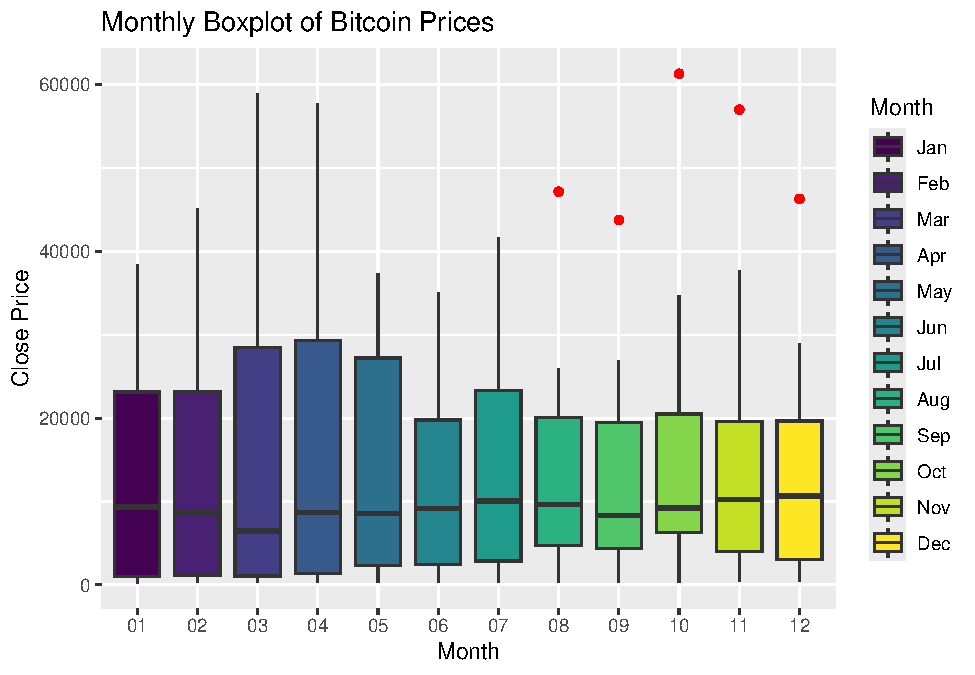
\includegraphics{bookdown-demo_files/figure-latex/unnamed-chunk-9-1.pdf}

\emph{\textbf{Code explanation here}}

\begin{itemize}
\tightlist
\item
  The boxplot shows that Bitcoin prices exhibit some level of seasonal variation.
\item
  Prices tend to be higher during certain months (March, April, May) compared to others ( June, July).
\item
  This could indicate seasonal trends or cycles in the market.
\item
  The presence of outliers (red dots) in some months, especially in May and September, indicates that there were extreme price changes during these periods.
\end{itemize}

\section*{Create a yearly boxplot of prices.}\label{create-a-yearly-boxplot-of-prices.}
\addcontentsline{toc}{section}{Create a yearly boxplot of prices.}

\begin{Shaded}
\begin{Highlighting}[]
\FunctionTok{library}\NormalTok{(RColorBrewer)}

\CommentTok{\# 2. Create a yearly boxplot of prices}
\NormalTok{color\_palette }\OtherTok{\textless{}{-}} \FunctionTok{brewer.pal}\NormalTok{(}\DecValTok{9}\NormalTok{, }\StringTok{"Set3"}\NormalTok{)  }\CommentTok{\# 9 colors for 9 years}

\CommentTok{\#the boxplot with a legend for the years}
\FunctionTok{ggplot}\NormalTok{(BitCoin\_df, }\FunctionTok{aes}\NormalTok{(}\AttributeTok{x =} \FunctionTok{factor}\NormalTok{(year), }\AttributeTok{y =}\NormalTok{ Close, }\AttributeTok{fill =} \FunctionTok{factor}\NormalTok{(year))) }\SpecialCharTok{+}
  \FunctionTok{geom\_boxplot}\NormalTok{(}\AttributeTok{outlier.colour =} \StringTok{"red"}\NormalTok{) }\SpecialCharTok{+}
  \FunctionTok{labs}\NormalTok{(}\AttributeTok{title =} \StringTok{"Yearly Boxplot of Bitcoin Prices"}\NormalTok{, }\AttributeTok{x =} \StringTok{"Year"}\NormalTok{, }\AttributeTok{y =} \StringTok{"Close Price"}\NormalTok{) }\SpecialCharTok{+}
  \FunctionTok{scale\_fill\_manual}\NormalTok{(}\AttributeTok{name =} \StringTok{"Year"}\NormalTok{, }\AttributeTok{values =} \FunctionTok{setNames}\NormalTok{(color\_palette, }\FunctionTok{as.character}\NormalTok{(}\DecValTok{2015}\SpecialCharTok{:}\DecValTok{2023}\NormalTok{))) }\SpecialCharTok{+}
  \FunctionTok{theme}\NormalTok{(}\AttributeTok{legend.position =} \StringTok{"right"}\NormalTok{)}
\end{Highlighting}
\end{Shaded}

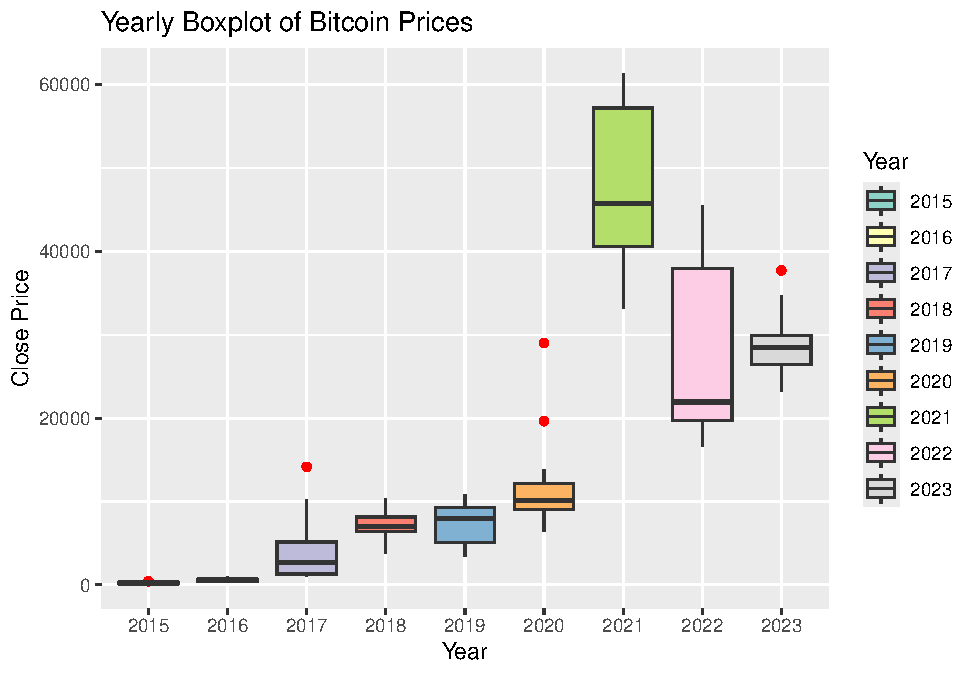
\includegraphics{bookdown-demo_files/figure-latex/unnamed-chunk-10-1.pdf}

\emph{\textbf{Code explanation here}}

\begin{itemize}
\tightlist
\item
  A boxplot showing the distribution of Bitcoin closing prices over different years.
\item
  Each box represents the interquartile range (IQR) of the closing prices for a particular year, with the horizontal line inside the box indicating the median price. T
\item
  he whiskers extend to the minimum and maximum values within 1.5 times the IQR from the first and third quartiles, respectively.
\item
  Outliers beyond this range are shown as individual points.
\end{itemize}

\section*{Create year wise trend lines of prices.}\label{create-year-wise-trend-lines-of-prices.}
\addcontentsline{toc}{section}{Create year wise trend lines of prices.}

\begin{Shaded}
\begin{Highlighting}[]
\CommentTok{\# 3. Create year{-}wise trend lines of prices}
\FunctionTok{ggplot}\NormalTok{(BitCoin\_df, }\FunctionTok{aes}\NormalTok{(}\AttributeTok{x =}\NormalTok{ Date, }\AttributeTok{y =}\NormalTok{ Close, }\AttributeTok{color =}\NormalTok{ year)) }\SpecialCharTok{+}
  \FunctionTok{geom\_line}\NormalTok{() }\SpecialCharTok{+}
  \FunctionTok{labs}\NormalTok{(}\AttributeTok{title =} \StringTok{"Year{-}Wise Trend Lines of Bitcoin Prices"}\NormalTok{, }\AttributeTok{x =} \StringTok{"Date"}\NormalTok{, }\AttributeTok{y =} \StringTok{"Close Price"}\NormalTok{) }\SpecialCharTok{+}
  \FunctionTok{theme}\NormalTok{(}\AttributeTok{legend.position =} \StringTok{"bottom"}\NormalTok{)}
\end{Highlighting}
\end{Shaded}

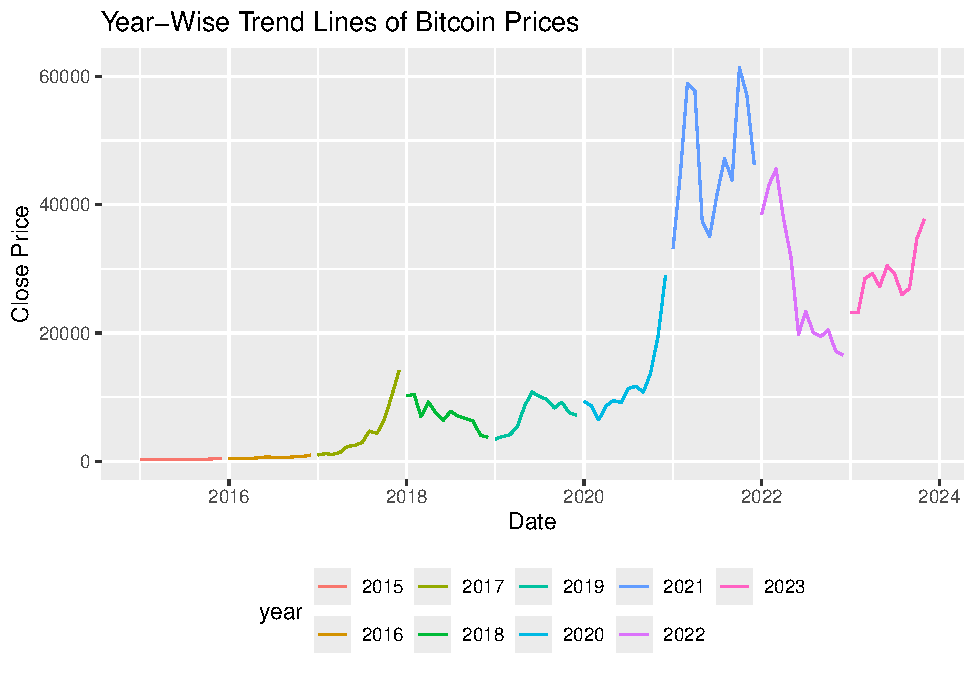
\includegraphics{bookdown-demo_files/figure-latex/unnamed-chunk-11-1.pdf}

\emph{\textbf{Explanation of Plot}}

\begin{itemize}
\tightlist
\item
  A trend line showing the price of Bitcoin changes over different years.
\item
  2015,2016: Bitcoin prices were relatively low and stable, with prices mostly below \$1,000.
\item
  2017: Significant growth was observed, with prices starting below \$1,000 and rising to nearly \$20,000 by the end of the year.
\item
  2018,2019: After the peak in 2017, prices dropped significantly, fluctuating between \$3,000 and \$10,000.Prices started to recover, stabilizing between \$3,000 and \$12,000.
\item
  2020: There was a steady increase, with prices rising from around \$5,000 to over \$30,000 by the end of the year.
\item
  2021: Marked a dramatic rise, with Bitcoin prices reaching new all-time highs, peaking around \$60,000.
\item
  2022: Prices were highly volatile, with significant drops and recoveries, ranging from \$30,000 to \$50,000.
\item
  2023: Prices appeared to stabilize somewhat, fluctuating between \$20,000 and \$40,000.
\end{itemize}

\subsection*{Convert the BitCoin data frame to a time series object with frequency 1}\label{convert-the-bitcoin-data-frame-to-a-time-series-object-with-frequency-1}
\addcontentsline{toc}{subsection}{Convert the BitCoin data frame to a time series object with frequency 1}

\begin{Shaded}
\begin{Highlighting}[]
\CommentTok{\# Convert the BitCoin data frame to a time series object with frequency 1}
\NormalTok{bitcoin\_ts }\OtherTok{\textless{}{-}} \FunctionTok{ts}\NormalTok{(BitCoin\_df}\SpecialCharTok{$}\NormalTok{Close, }\AttributeTok{start =} \FunctionTok{c}\NormalTok{(}\FunctionTok{as.numeric}\NormalTok{(}\FunctionTok{format}\NormalTok{(}\FunctionTok{min}\NormalTok{(BitCoin\_df}\SpecialCharTok{$}\NormalTok{Date), }\StringTok{"\%Y"}\NormalTok{)), }\DecValTok{1}\NormalTok{), }\AttributeTok{frequency =} \DecValTok{1}\NormalTok{)}

\CommentTok{\# Print the time series object}
\FunctionTok{print}\NormalTok{(bitcoin\_ts)}
\end{Highlighting}
\end{Shaded}

\begin{verbatim}
## Time Series:
## Start = 2015 
## End = 2121 
## Frequency = 1 
##   [1]   217.464   254.263   244.224   236.145   230.190   263.072   284.650
##   [8]   230.056   236.060   314.166   377.321   430.567   368.767   437.697
##  [15]   416.729   448.318   531.386   673.337   624.681   575.472   609.735
##  [22]   700.972   745.691   963.743   970.403  1179.970  1071.790  1347.890
##  [29]  2286.410  2480.840  2875.340  4703.390  4338.710  6468.400 10233.600
##  [36] 14156.400 10221.100 10397.900  6973.530  9240.550  7494.170  6404.000
##  [43]  7780.440  7037.580  6625.560  6317.610  4017.269  3742.700  3457.793
##  [50]  3854.785  4105.404  5350.727  8574.502 10817.155 10085.628  9630.664
##  [57]  8293.868  9199.585  7569.630  7193.599  9350.529  8599.509  6438.645
##  [64]  8658.554  9461.059  9137.993 11323.467 11680.820 10784.491 13780.995
##  [71] 19625.836 29001.721 33114.359 45137.770 58918.832 57750.176 37332.855
##  [78] 35040.836 41626.195 47166.688 43790.895 61318.957 57005.426 46306.445
##  [85] 38483.125 43193.234 45538.676 37714.875 31792.311 19784.727 23336.896
##  [92] 20049.764 19431.789 20495.773 17168.566 16547.496 23139.283 23147.354
##  [99] 28478.484 29268.807 27219.658 30477.252 29230.111 25931.473 26967.916
## [106] 34667.781 37712.746
\end{verbatim}

\subsection*{Plot the time series of monthly prices on years. Use blue color dots to plot the data points. Connect the points with a line.}\label{plot-the-time-series-of-monthly-prices-on-years.-use-blue-color-dots-to-plot-the-data-points.-connect-the-points-with-a-line.}
\addcontentsline{toc}{subsection}{Plot the time series of monthly prices on years. Use blue color dots to plot the data points. Connect the points with a line.}

\begin{Shaded}
\begin{Highlighting}[]
\CommentTok{\# Plot the time series of monthly prices on years}
\FunctionTok{ggplot}\NormalTok{(BitCoin\_df, }\FunctionTok{aes}\NormalTok{(}\AttributeTok{x =}\NormalTok{ Date, }\AttributeTok{y =}\NormalTok{ Close)) }\SpecialCharTok{+}
  \FunctionTok{geom\_point}\NormalTok{(}\AttributeTok{color =} \StringTok{"blue"}\NormalTok{) }\SpecialCharTok{+} \CommentTok{\# Blue color dots for data points}
  \FunctionTok{geom\_line}\NormalTok{(}\AttributeTok{color =} \StringTok{"blue"}\NormalTok{) }\SpecialCharTok{+}  \CommentTok{\# Connect the points with a line}
  \FunctionTok{labs}\NormalTok{(}\AttributeTok{title =} \StringTok{"Time Series of Monthly Bitcoin Prices"}\NormalTok{,}
       \AttributeTok{x =} \StringTok{"Year"}\NormalTok{,}
       \AttributeTok{y =} \StringTok{"Close Price"}\NormalTok{) }\SpecialCharTok{+}
  \FunctionTok{theme\_minimal}\NormalTok{()}
\end{Highlighting}
\end{Shaded}

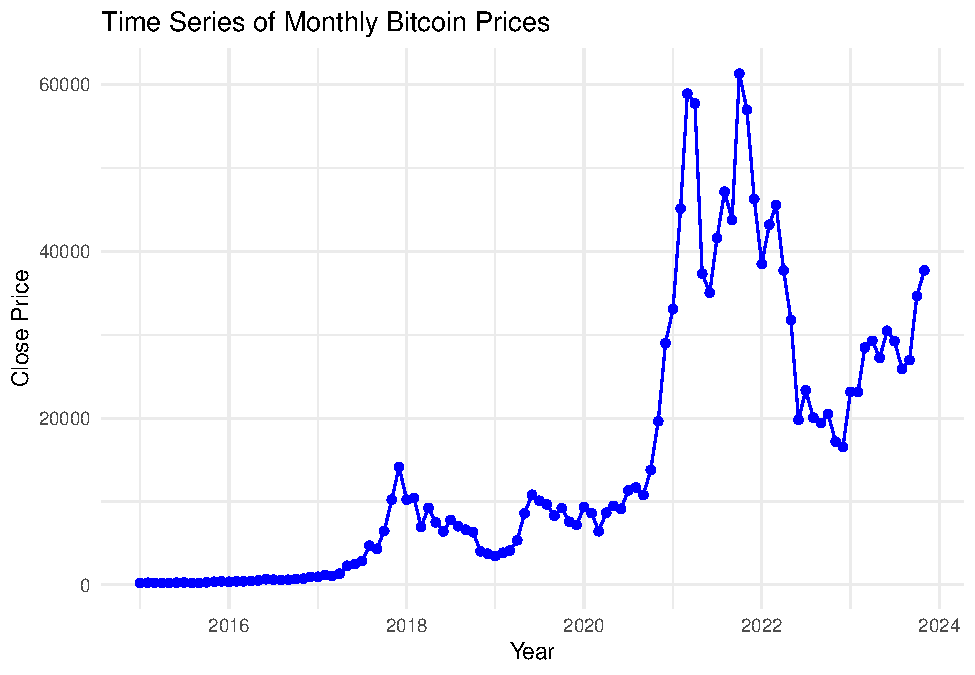
\includegraphics{bookdown-demo_files/figure-latex/unnamed-chunk-13-1.pdf}

\emph{\textbf{Explanation of Plot}}

Explanation of the Plot:

\begin{itemize}
\tightlist
\item
  Horizontal Axis (Year): Represents the timeline from 2016 to 2024.
\item
  Vertical Axis (Close Price): Represents the closing price of Bitcoin at the end of each month.
\item
  Blue Dots: Each dot represents the closing price of Bitcoin for a particular month.
\item
  Blue Line: Connects the dots to show the trend and continuity of Bitcoin prices over time.
\item
  The plot provides a visual representation of Bitcoin's price volatility and trends, making it easier to analyze patterns and potential factors affecting its value over the given period.
\end{itemize}

\emph{\textbf{Result}}

The plot reveals significant fluctuations in Bitcoin prices, including notable peaks around 2021 and subsequent declines. The most recent data indicates a rising trend in prices again.

\section*{Find the relationship between consecutive months. Show the correlation through a scatter plot.}\label{find-the-relationship-between-consecutive-months.-show-the-correlation-through-a-scatter-plot.}
\addcontentsline{toc}{section}{Find the relationship between consecutive months. Show the correlation through a scatter plot.}

\begin{Shaded}
\begin{Highlighting}[]
\FunctionTok{library}\NormalTok{(dplyr)}
\FunctionTok{library}\NormalTok{(ggplot2)}
\FunctionTok{library}\NormalTok{(lubridate)}

\CommentTok{\# Aggregate the data by month}
\NormalTok{BitCoin\_df\_monthly }\OtherTok{\textless{}{-}}\NormalTok{ BitCoin\_df }\SpecialCharTok{\%\textgreater{}\%}
  \FunctionTok{mutate}\NormalTok{(}\AttributeTok{YearMonth =} \FunctionTok{floor\_date}\NormalTok{(Date, }\StringTok{"month"}\NormalTok{)) }\SpecialCharTok{\%\textgreater{}\%}
  \FunctionTok{group\_by}\NormalTok{(YearMonth) }\SpecialCharTok{\%\textgreater{}\%}
  \FunctionTok{summarise}\NormalTok{(}\AttributeTok{Monthly\_Close =} \FunctionTok{last}\NormalTok{(Close)) }\SpecialCharTok{\%\textgreater{}\%}
  \FunctionTok{arrange}\NormalTok{(YearMonth)}

\CommentTok{\# Create a new column for the previous month\textquotesingle{}s closing price}
\NormalTok{BitCoin\_df\_monthly }\OtherTok{\textless{}{-}}\NormalTok{ BitCoin\_df\_monthly }\SpecialCharTok{\%\textgreater{}\%}
  \FunctionTok{mutate}\NormalTok{(}\AttributeTok{Prev\_Month\_Close =} \FunctionTok{lag}\NormalTok{(Monthly\_Close, }\DecValTok{1}\NormalTok{))}

\CommentTok{\# Remove the first row with NA value in Prev\_Month\_Close}
\NormalTok{BitCoin\_df\_monthly }\OtherTok{\textless{}{-}}\NormalTok{ BitCoin\_df\_monthly }\SpecialCharTok{\%\textgreater{}\%}
  \FunctionTok{filter}\NormalTok{(}\SpecialCharTok{!}\FunctionTok{is.na}\NormalTok{(Prev\_Month\_Close))}

\CommentTok{\# Calculate the correlation}
\NormalTok{monthly\_correlation }\OtherTok{\textless{}{-}} \FunctionTok{cor}\NormalTok{(BitCoin\_df\_monthly}\SpecialCharTok{$}\NormalTok{Monthly\_Close, BitCoin\_df\_monthly}\SpecialCharTok{$}\NormalTok{Prev\_Month\_Close)}
\FunctionTok{print}\NormalTok{(}\FunctionTok{paste}\NormalTok{(}\StringTok{"Correlation between consecutive months: "}\NormalTok{, monthly\_correlation))}
\end{Highlighting}
\end{Shaded}

\begin{verbatim}
## [1] "Correlation between consecutive months:  0.961776393506846"
\end{verbatim}

\begin{Shaded}
\begin{Highlighting}[]
\CommentTok{\# Create a scatter plot}
\FunctionTok{ggplot}\NormalTok{(BitCoin\_df\_monthly, }\FunctionTok{aes}\NormalTok{(}\AttributeTok{x =}\NormalTok{ Prev\_Month\_Close, }\AttributeTok{y =}\NormalTok{ Monthly\_Close)) }\SpecialCharTok{+}
  \FunctionTok{geom\_point}\NormalTok{(}\AttributeTok{color =} \StringTok{"blue"}\NormalTok{) }\SpecialCharTok{+}
  \FunctionTok{labs}\NormalTok{(}\AttributeTok{title =} \StringTok{"Scatter Plot of Consecutive Month Prices"}\NormalTok{,}
       \AttributeTok{subtitle =} \FunctionTok{paste}\NormalTok{(}\StringTok{"Correlation: "}\NormalTok{, }\FunctionTok{round}\NormalTok{(monthly\_correlation, }\DecValTok{2}\NormalTok{)),}
       \AttributeTok{x =} \StringTok{"Previous Month Close Price"}\NormalTok{,}
       \AttributeTok{y =} \StringTok{"Current Month Close Price"}\NormalTok{) }\SpecialCharTok{+}
  \FunctionTok{theme\_minimal}\NormalTok{()}
\end{Highlighting}
\end{Shaded}

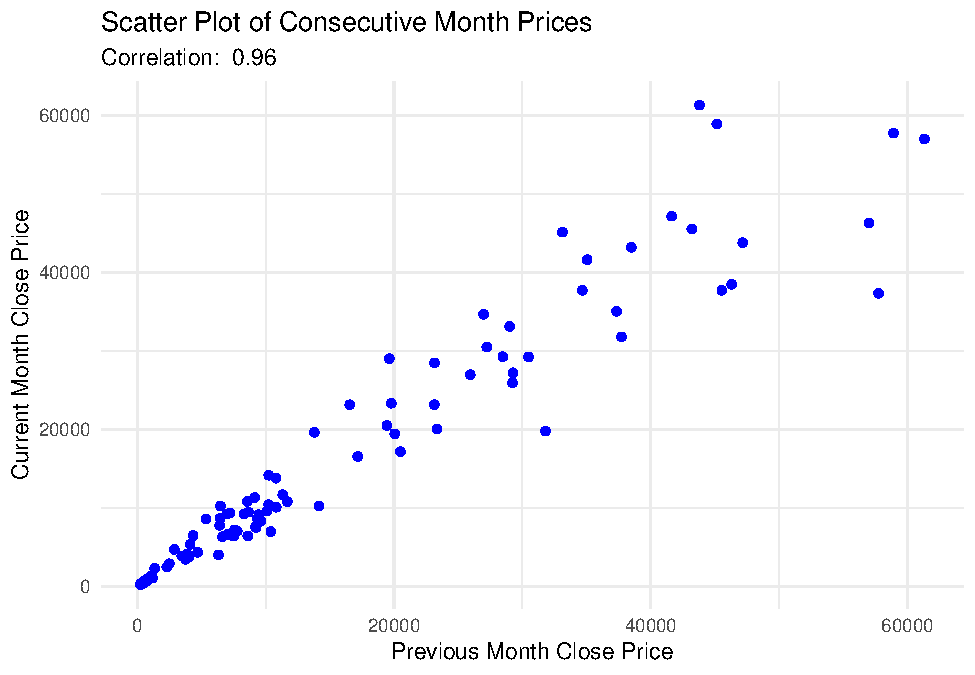
\includegraphics{bookdown-demo_files/figure-latex/unnamed-chunk-14-1.pdf}

\emph{\textbf{Code explanation here}}

The scatter plot provides a clear visual representation of the relationship between Bitcoin prices in consecutive months, highlighting the strong correlation 0.96 and linear trend, which are valuable for analyses and decision-making processes.

\begin{itemize}
\tightlist
\item
  Horizontal Axis (Previous Month Close Price): Represents the closing price of Bitcoin for the previous month.
\item
  Vertical Axis (Current Month Close Price): Represents the closing price of Bitcoin for the current month.
\item
  Blue Dots: Each dot represents the closing price of Bitcoin for a specific month plotted against the closing price of the previous month.
\item
  Correlation Value: Displayed at the top of the chart, it quantifies the strength of the relationship between - consecutive month's prices.
\end{itemize}

\chapter{Regression Analysis}\label{regression-analysis}

\subsection{Linear Regression}\label{linear-regression}

\begin{itemize}
\tightlist
\item
  Create a linear model of the time series dataset.
\item
  Show the summary of the model and explain the outcome.
\item
  Create a plot of the linear model on top of the time series dataset line plot with scatter data points.
\item
  Perform residual analysis and create a line \& scatter plot of the residuals. Explain the outcome.
\item
  Create a histogram plot of the residuals. Explain the outcome.
\item
  Create ACF \& PACF plots of residuals. Explain the outcome.
\item
  Create QQ plot of residuals. Explain the outcome.
\item
  Perform Shapiro-Wilk test on residuals. Explain the outcome.
\item
  Explain if linear model is appropriate or not.
\end{itemize}

\subsubsection{Create a linear model of the time series dataset.}\label{create-a-linear-model-of-the-time-series-dataset.}

\begin{Shaded}
\begin{Highlighting}[]
\CommentTok{\# Convert Date to numeric format for linear modeling}
\NormalTok{BitCoin\_df }\OtherTok{\textless{}{-}}\NormalTok{ BitCoin\_df }\SpecialCharTok{\%\textgreater{}\%}
\FunctionTok{mutate}\NormalTok{(}\AttributeTok{Date\_numeric =} \FunctionTok{as.numeric}\NormalTok{(Date))}

\CommentTok{\# Fit the linear model}
\NormalTok{linear\_model }\OtherTok{\textless{}{-}} \FunctionTok{lm}\NormalTok{(Close }\SpecialCharTok{\textasciitilde{}}\NormalTok{ Date\_numeric, }\AttributeTok{data =}\NormalTok{ BitCoin\_df)}
\CommentTok{\#y=mx+c}
\CommentTok{\#close price = m*numeric date + c}
\end{Highlighting}
\end{Shaded}

\emph{\textbf{Code explanation here}}
The linear model predicts Bitcoin's closing price based on the date. The slope shows the price change rate over time, and the intercept represents the initial price at the start date.

\subsubsection{Show the summary of the model and explain the outcome.}\label{show-the-summary-of-the-model-and-explain-the-outcome.}

\begin{Shaded}
\begin{Highlighting}[]
\FunctionTok{summary}\NormalTok{(linear\_model)}
\end{Highlighting}
\end{Shaded}

\begin{verbatim}
## 
## Call:
## lm(formula = Close ~ Date_numeric, data = BitCoin_df)
## 
## Residuals:
##    Min     1Q Median     3Q    Max 
## -15114  -7997  -2255   3065  35626 
## 
## Coefficients:
##                Estimate Std. Error t value Pr(>|t|)    
## (Intercept)  -2.211e+05  1.939e+04  -11.40   <2e-16 ***
## Date_numeric  1.308e+01  1.073e+00   12.19   <2e-16 ***
## ---
## Signif. codes:  0 '***' 0.001 '**' 0.01 '*' 0.05 '.' 0.1 ' ' 1
## 
## Residual standard error: 10430 on 105 degrees of freedom
## Multiple R-squared:  0.586,  Adjusted R-squared:  0.5821 
## F-statistic: 148.6 on 1 and 105 DF,  p-value: < 2.2e-16
\end{verbatim}

\emph{\textbf{In Summary}}

\begin{itemize}
\tightlist
\item
  The model indicates a statistically significant relationship between the date and the closing price of Bitcoin, as shown by the very small p-value (\textless{} 2.2e-16).
\item
  The date explains about 58.6\% of the variation in closing prices, as reflected by the Multiple R-squared and Adjusted R-squared values.
\item
  The average prediction error is approximately 10430, as indicated by the Residual Standard Error.
\item
  For each unit increase in the numeric date, the closing price of Bitcoin rises by about 13.08 units, which is determined by the slope of the regression line.
\end{itemize}

\begin{Shaded}
\begin{Highlighting}[]
\CommentTok{\# Create a new column with fitted values}
\NormalTok{BitCoin\_df }\OtherTok{\textless{}{-}}\NormalTok{ BitCoin\_df }\SpecialCharTok{\%\textgreater{}\%}
\FunctionTok{mutate}\NormalTok{(}\AttributeTok{Fitted\_Close =} \FunctionTok{predict}\NormalTok{(linear\_model))}

\CommentTok{\# Plot the original data and the linear model}

\FunctionTok{ggplot}\NormalTok{(BitCoin\_df, }\FunctionTok{aes}\NormalTok{(}\AttributeTok{x =}\NormalTok{ Date)) }\SpecialCharTok{+}
\FunctionTok{geom\_point}\NormalTok{(}\FunctionTok{aes}\NormalTok{(}\AttributeTok{y =}\NormalTok{ Close, }\AttributeTok{color =} \StringTok{"Original Data"}\NormalTok{)) }\SpecialCharTok{+}  \CommentTok{\# Original data points}
\FunctionTok{geom\_line}\NormalTok{(}\FunctionTok{aes}\NormalTok{(}\AttributeTok{y =}\NormalTok{ Fitted\_Close, }\AttributeTok{color =} \StringTok{"Fitted Line"}\NormalTok{)) }\SpecialCharTok{+}  \CommentTok{\# Fitted line}
\FunctionTok{labs}\NormalTok{(}\AttributeTok{title =} \StringTok{"Linear Model of Bitcoin Prices Over Time"}\NormalTok{,}
     \AttributeTok{x =} \StringTok{"Date"}\NormalTok{,}
     \AttributeTok{y =} \StringTok{"Close Price"}\NormalTok{,}
     \AttributeTok{color =} \StringTok{"Legend"}\NormalTok{) }\SpecialCharTok{+}  \CommentTok{\# Add a label to the legend}
\FunctionTok{theme\_minimal}\NormalTok{() }\SpecialCharTok{+}
\FunctionTok{scale\_color\_manual}\NormalTok{(}\AttributeTok{values =} \FunctionTok{c}\NormalTok{(}\StringTok{"Original Data"} \OtherTok{=} \StringTok{"blue"}\NormalTok{, }\StringTok{"Fitted Line"} \OtherTok{=} \StringTok{"red"}\NormalTok{))  }\CommentTok{\# Specify colors}
\end{Highlighting}
\end{Shaded}

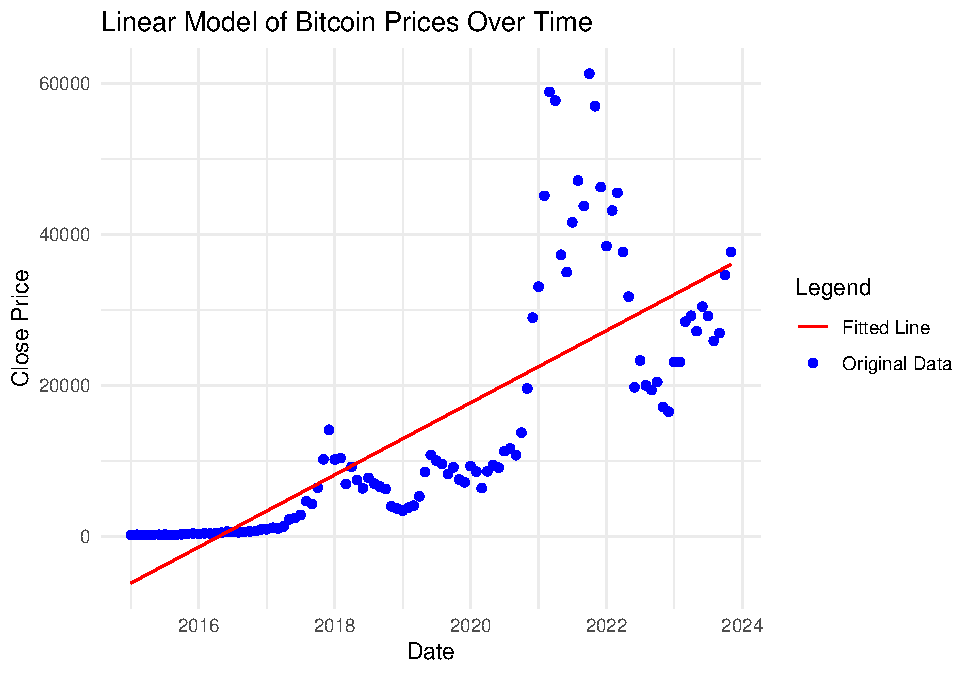
\includegraphics{bookdown-demo_files/figure-latex/unnamed-chunk-18-1.pdf}

\emph{\textbf{Code explanation here}}

The provided graph and summary show a linear regression model of Bitcoin prices over time. The blue points represent the original data, while the red line represents the fitted linear model.

\subsubsection{Create a plot of the linear model on top of the time series dataset line plot with scatter data points.}\label{create-a-plot-of-the-linear-model-on-top-of-the-time-series-dataset-line-plot-with-scatter-data-points.}

\begin{Shaded}
\begin{Highlighting}[]
\CommentTok{\#Create a plot of the linear model on top of the time series dataset line plot with scatter data points.}
  
\CommentTok{\#Plot the original data, the time series line, and the linear model}
\FunctionTok{ggplot}\NormalTok{(BitCoin\_df, }\FunctionTok{aes}\NormalTok{(}\AttributeTok{x =}\NormalTok{ Date)) }\SpecialCharTok{+}
\FunctionTok{geom\_point}\NormalTok{(}\FunctionTok{aes}\NormalTok{(}\AttributeTok{y =}\NormalTok{ Close), }\AttributeTok{color =} \StringTok{"blue"}\NormalTok{) }\SpecialCharTok{+}  \CommentTok{\# Original data points}
\FunctionTok{geom\_line}\NormalTok{(}\FunctionTok{aes}\NormalTok{(}\AttributeTok{y =}\NormalTok{ Close), }\AttributeTok{color =} \StringTok{"blue"}\NormalTok{, }\AttributeTok{linetype =} \StringTok{"dashed"}\NormalTok{) }\SpecialCharTok{+}  \CommentTok{\# Time series line}
\FunctionTok{geom\_line}\NormalTok{(}\FunctionTok{aes}\NormalTok{(}\AttributeTok{y =}\NormalTok{ Fitted\_Close), }\AttributeTok{color =} \StringTok{"red"}\NormalTok{) }\SpecialCharTok{+}  \CommentTok{\# Fitted linear model line}
\FunctionTok{labs}\NormalTok{(}\AttributeTok{title =} \StringTok{"Time Series of Bitcoin Prices with Linear Model"}\NormalTok{,}
     \AttributeTok{x =} \StringTok{"Date"}\NormalTok{,}
     \AttributeTok{y =} \StringTok{"Close Price"}\NormalTok{) }\SpecialCharTok{+}
\FunctionTok{theme\_minimal}\NormalTok{() }
\end{Highlighting}
\end{Shaded}

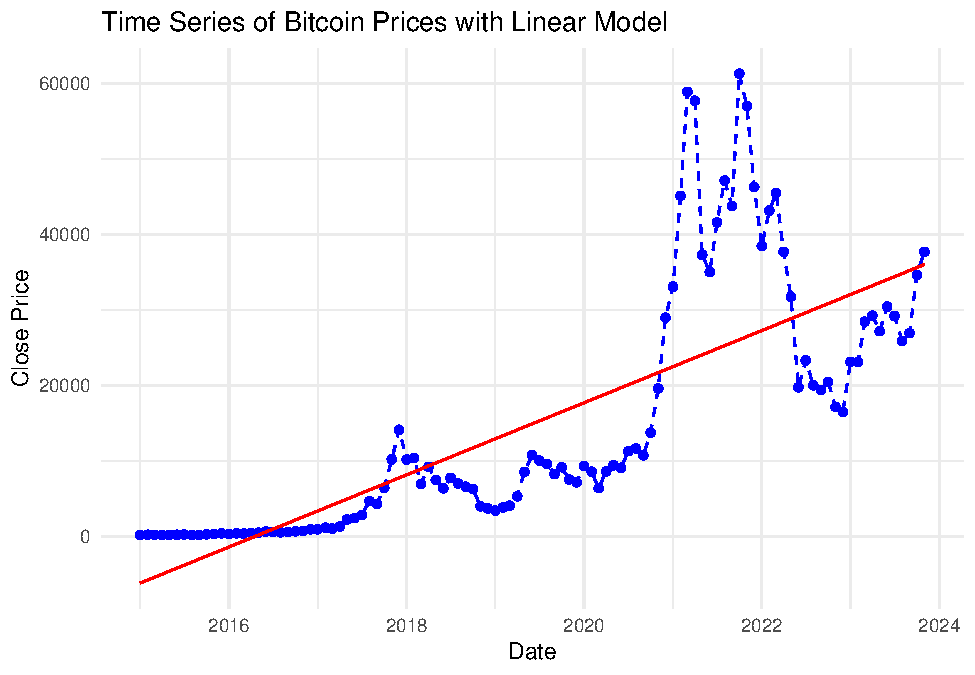
\includegraphics{bookdown-demo_files/figure-latex/unnamed-chunk-19-1.pdf}

\emph{\textbf{Code explanation here}}
The graph shows Bitcoin prices over time with blue dots representing the original data points and a blue dashed line representing the time series trend. The red line indicates the fitted linear model. The linear model captures the general upward trend but misses some of the more volatile fluctuations in Bitcoin prices.

\subsubsection{Perform residual analysis}\label{perform-residual-analysis}

\begin{Shaded}
\begin{Highlighting}[]
\CommentTok{\#Calculate residuals}
\NormalTok{BitCoin\_df }\OtherTok{\textless{}{-}}\NormalTok{ BitCoin\_df }\SpecialCharTok{\%\textgreater{}\%}
\FunctionTok{mutate}\NormalTok{(}\AttributeTok{Residuals =}\NormalTok{ Close }\SpecialCharTok{{-}}\NormalTok{ Fitted\_Close)}

\CommentTok{\#residual calcultion in different way}
\CommentTok{\#res\_dual\_values \textless{}{-} residuals(linear\_model)}
\CommentTok{\#summary(res\_dual\_values)}
\end{Highlighting}
\end{Shaded}

\emph{\textbf{Code explanation here}}

Residuals are calculated to assess model fit. The dataset includes date, closing price, month, year, numeric date, fitted close values, and residuals for verification.

\subsubsection{Perform residual analysis and create a line \& scatter plot of the}\label{perform-residual-analysis-and-create-a-line-scatter-plot-of-the}

\begin{Shaded}
\begin{Highlighting}[]
\CommentTok{\# Plot the residuals: Line plot}
\FunctionTok{ggplot}\NormalTok{(BitCoin\_df, }\FunctionTok{aes}\NormalTok{(}\AttributeTok{x =}\NormalTok{ Date, }\AttributeTok{y =}\NormalTok{ Residuals)) }\SpecialCharTok{+}
  \FunctionTok{geom\_line}\NormalTok{(}\AttributeTok{color =} \StringTok{"blue"}\NormalTok{) }\SpecialCharTok{+}
  \FunctionTok{labs}\NormalTok{(}\AttributeTok{title =} \StringTok{"Line Plot of Residuals over Time"}\NormalTok{,}
       \AttributeTok{x =} \StringTok{"Date"}\NormalTok{,}
       \AttributeTok{y =} \StringTok{"Residuals"}\NormalTok{) }\SpecialCharTok{+}
  \FunctionTok{theme\_minimal}\NormalTok{()}
\end{Highlighting}
\end{Shaded}

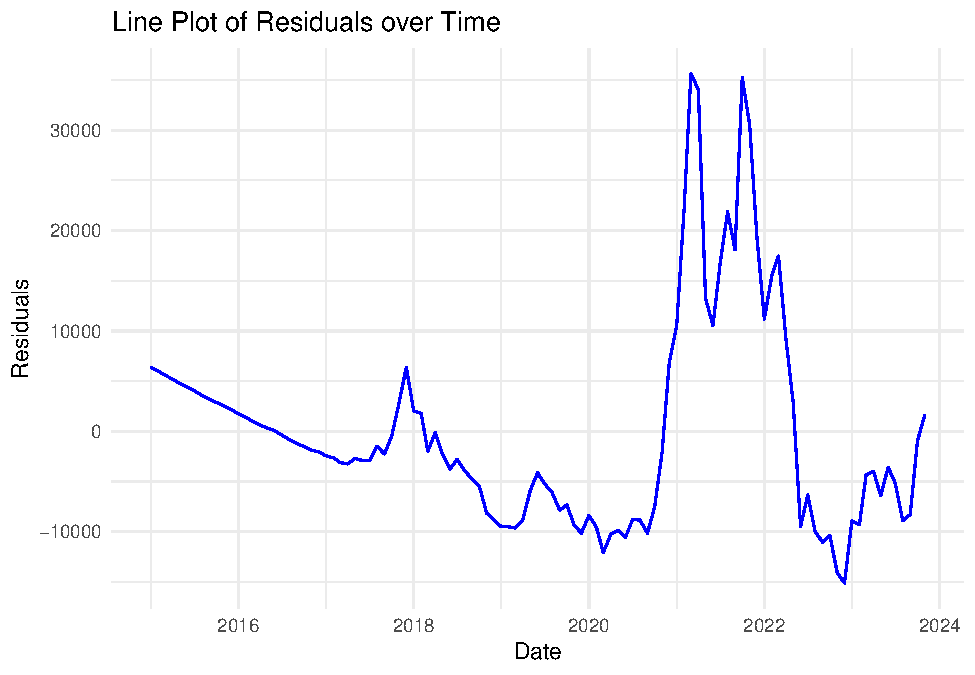
\includegraphics{bookdown-demo_files/figure-latex/unnamed-chunk-21-1.pdf}

\emph{\textbf{Code explanation here}}
The graph shows a blue line plotting the difference between actual values and predicted values for a Bitcoin data set, over time. Basically, it shows how much the actual Bitcoin values differed from what a model predicted on certain dates.

\subsubsection{Residual analysis scatter plot}\label{residual-analysis-scatter-plot}

\begin{Shaded}
\begin{Highlighting}[]
\CommentTok{\# Plot the residuals: Scatter plot}
\FunctionTok{ggplot}\NormalTok{(BitCoin\_df, }\FunctionTok{aes}\NormalTok{(}\AttributeTok{x =}\NormalTok{ Fitted\_Close, }\AttributeTok{y =}\NormalTok{ Residuals)) }\SpecialCharTok{+}
  \FunctionTok{geom\_point}\NormalTok{(}\AttributeTok{color =} \StringTok{"blue"}\NormalTok{) }\SpecialCharTok{+}
  \FunctionTok{geom\_hline}\NormalTok{(}\AttributeTok{yintercept =} \DecValTok{0}\NormalTok{, }\AttributeTok{linetype =} \StringTok{"dashed"}\NormalTok{, }\AttributeTok{color =} \StringTok{"red"}\NormalTok{) }\SpecialCharTok{+}
  \FunctionTok{labs}\NormalTok{(}\AttributeTok{title =} \StringTok{"Scatter Plot of Residuals"}\NormalTok{,}
       \AttributeTok{x =} \StringTok{"Fitted Close Price"}\NormalTok{,}
       \AttributeTok{y =} \StringTok{"Residuals"}\NormalTok{) }\SpecialCharTok{+}
  \FunctionTok{theme\_minimal}\NormalTok{()}
\end{Highlighting}
\end{Shaded}

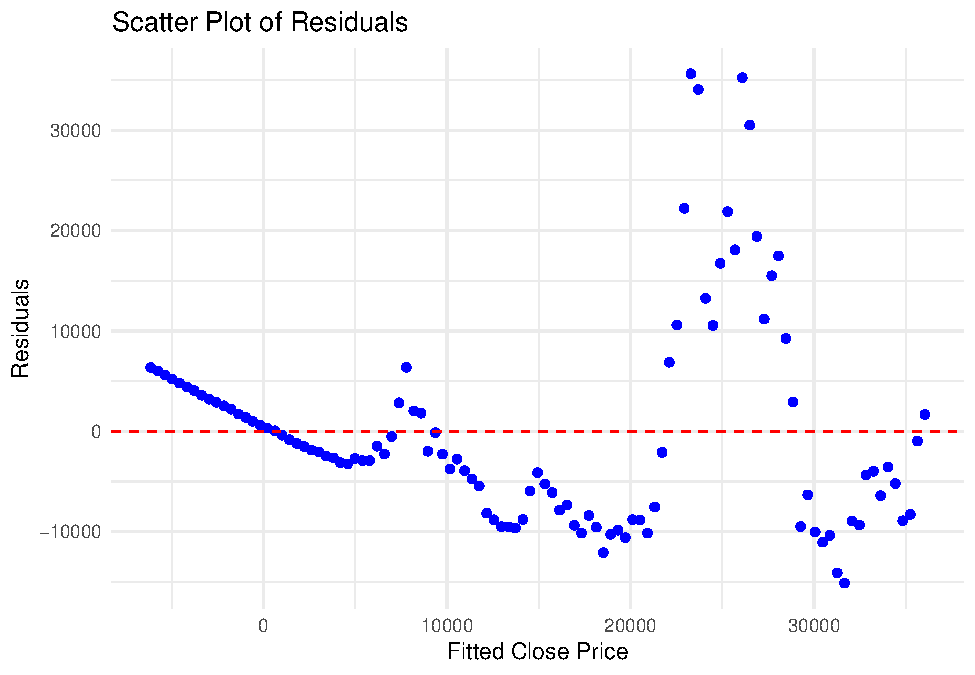
\includegraphics{bookdown-demo_files/figure-latex/unnamed-chunk-22-1.pdf}

\emph{\textbf{Code explanation here}}

This graph shows blue dots representing the difference between actual Bitcoin closing prices and what a model predicted. The horizontal red line represents perfect predictions (no difference). Scattered points around the line indicate the model's accuracy - ideally, the dots would be random with no clear pattern.

\subsubsection{Summary of Residual analysis}\label{summary-of-residual-analysis}

\begin{Shaded}
\begin{Highlighting}[]
\CommentTok{\# Summary statistics of the residuals}
\FunctionTok{summary}\NormalTok{(BitCoin\_df}\SpecialCharTok{$}\NormalTok{Residuals)  }
\end{Highlighting}
\end{Shaded}

\begin{verbatim}
##    Min. 1st Qu.  Median    Mean 3rd Qu.    Max. 
##  -15114   -7997   -2255       0    3065   35626
\end{verbatim}

\emph{\textbf{Code explanation here}}

The summary statistics of the residuals provide insight into the accuracy of the linear model's predictions for Bitcoin closing prices. The residuals range from -15,114 to 35,626, indicating the model sometimes significantly underestimates or overestimates the actual prices. The median residual of -2,255 suggests that half of the predictions are off by less than this amount. The mean residual is 0, indicating that, on average, the model's predictions are unbiased. The first and third quartiles (-7,997 and 3,065) show that 50\% of the residuals fall within this range, highlighting the variability in prediction accuracy.

\subsubsection{Create a histogram plot of the residuals. Explain the outcome.}\label{create-a-histogram-plot-of-the-residuals.-explain-the-outcome.}

\begin{Shaded}
\begin{Highlighting}[]
\CommentTok{\#Create a histogram plot of the residuals. Explain the outcome.}
  \CommentTok{\# Plot the histogram of residuals}
  \FunctionTok{ggplot}\NormalTok{(BitCoin\_df, }\FunctionTok{aes}\NormalTok{(}\AttributeTok{x =}\NormalTok{ Residuals)) }\SpecialCharTok{+}
  \FunctionTok{geom\_histogram}\NormalTok{(}\AttributeTok{binwidth =} \DecValTok{500}\NormalTok{, }\AttributeTok{color =} \StringTok{"black"}\NormalTok{, }\AttributeTok{fill =} \StringTok{"blue"}\NormalTok{, }\AttributeTok{alpha =} \FloatTok{0.7}\NormalTok{) }\SpecialCharTok{+}
  \FunctionTok{labs}\NormalTok{(}\AttributeTok{title =} \StringTok{"Histogram of Residuals"}\NormalTok{,}
       \AttributeTok{x =} \StringTok{"Residuals"}\NormalTok{,}
       \AttributeTok{y =} \StringTok{"Frequency"}\NormalTok{) }\SpecialCharTok{+}
  \FunctionTok{theme\_minimal}\NormalTok{()}
\end{Highlighting}
\end{Shaded}

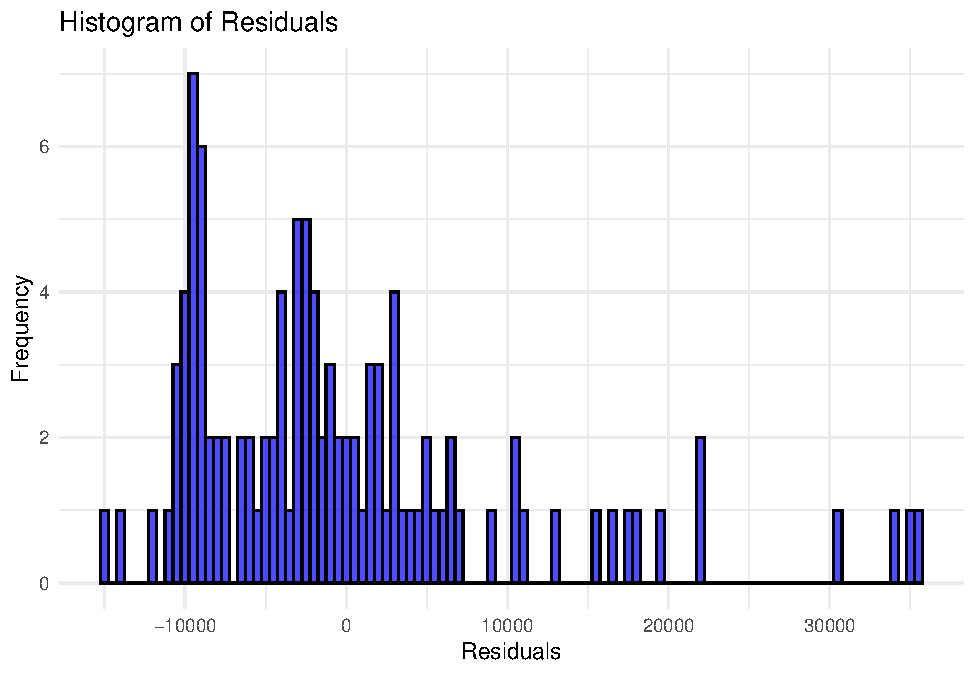
\includegraphics{bookdown-demo_files/figure-latex/unnamed-chunk-24-1.pdf}

\emph{\textbf{Code explanation here}}

Ideally, the residuals should be normally distributed (bell-shaped curve centered around zero).
The histogram here shows some deviation from normality, indicating that the model may not perfectly capture the data distribution.

\subsubsection{Create a histogram plot of the residuals with}\label{create-a-histogram-plot-of-the-residuals-with}

\begin{Shaded}
\begin{Highlighting}[]
\CommentTok{\# Overlay a normal distribution curve on the histogram}
\FunctionTok{ggplot}\NormalTok{(BitCoin\_df, }\FunctionTok{aes}\NormalTok{(}\AttributeTok{x =}\NormalTok{ Residuals)) }\SpecialCharTok{+}
  \FunctionTok{geom\_histogram}\NormalTok{(}\FunctionTok{aes}\NormalTok{(}\AttributeTok{y =}\NormalTok{ ..density..), }\AttributeTok{binwidth =} \DecValTok{500}\NormalTok{, }\AttributeTok{color =} \StringTok{"black"}\NormalTok{, }\AttributeTok{fill =} \StringTok{"blue"}\NormalTok{, }\AttributeTok{alpha =} \FloatTok{0.7}\NormalTok{) }\SpecialCharTok{+}
  \FunctionTok{stat\_function}\NormalTok{(}\AttributeTok{fun =}\NormalTok{ dnorm, }\AttributeTok{args =} \FunctionTok{list}\NormalTok{(}\AttributeTok{mean =} \FunctionTok{mean}\NormalTok{(BitCoin\_df}\SpecialCharTok{$}\NormalTok{Residuals), }\AttributeTok{sd =} \FunctionTok{sd}\NormalTok{(BitCoin\_df}\SpecialCharTok{$}\NormalTok{Residuals)), }\AttributeTok{color =} \StringTok{"red"}\NormalTok{, }\AttributeTok{size =} \DecValTok{1}\NormalTok{) }\SpecialCharTok{+}
  \FunctionTok{labs}\NormalTok{(}\AttributeTok{title =} \StringTok{"Histogram of Residuals with Normal Curve"}\NormalTok{,}
       \AttributeTok{x =} \StringTok{"Residuals"}\NormalTok{,}
       \AttributeTok{y =} \StringTok{"Density"}\NormalTok{) }\SpecialCharTok{+}
  \FunctionTok{theme\_minimal}\NormalTok{()}
\end{Highlighting}
\end{Shaded}

\begin{verbatim}
## Warning: Using `size` aesthetic for lines was deprecated in ggplot2 3.4.0.
## i Please use `linewidth` instead.
## This warning is displayed once every 8 hours.
## Call `lifecycle::last_lifecycle_warnings()` to see where this warning was
## generated.
\end{verbatim}

\begin{verbatim}
## Warning: The dot-dot notation (`..density..`) was deprecated in ggplot2 3.4.0.
## i Please use `after_stat(density)` instead.
## This warning is displayed once every 8 hours.
## Call `lifecycle::last_lifecycle_warnings()` to see where this warning was
## generated.
\end{verbatim}

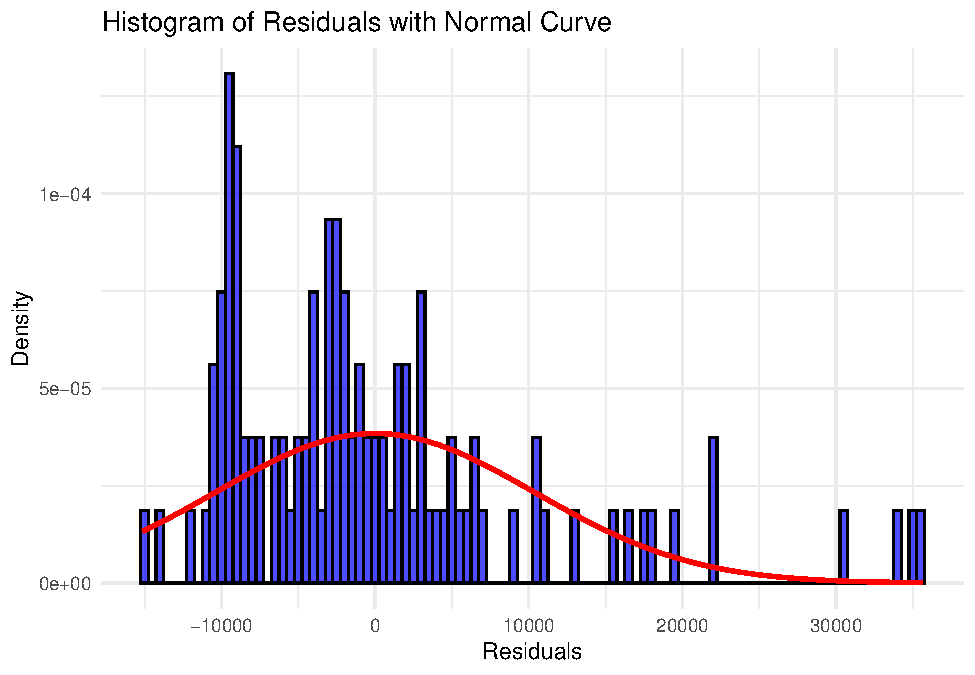
\includegraphics{bookdown-demo_files/figure-latex/unnamed-chunk-25-1.pdf}

\emph{\textbf{code explanation here}}

This graph shows a histogram of prediction errors (residuals) for Bitcoin prices with a normal distribution curve overlaid in red. The bars represent the frequency of errors in different price ranges. Ideally, the bars would closely match the smooth red curve, indicating the errors follow a normal distribution. By comparing their shapes, we can assess how close the actual errors are to being normally distributed.

\subsubsection{Create ACF \& PACF plots of residuals.Explain the outcome.}\label{create-acf-pacf-plots-of-residuals.explain-the-outcome.}

\begin{Shaded}
\begin{Highlighting}[]
\FunctionTok{acf}\NormalTok{(BitCoin\_df}\SpecialCharTok{$}\NormalTok{Residuals, }\AttributeTok{main =} \StringTok{"ACF of Residuals"}\NormalTok{)}
\end{Highlighting}
\end{Shaded}

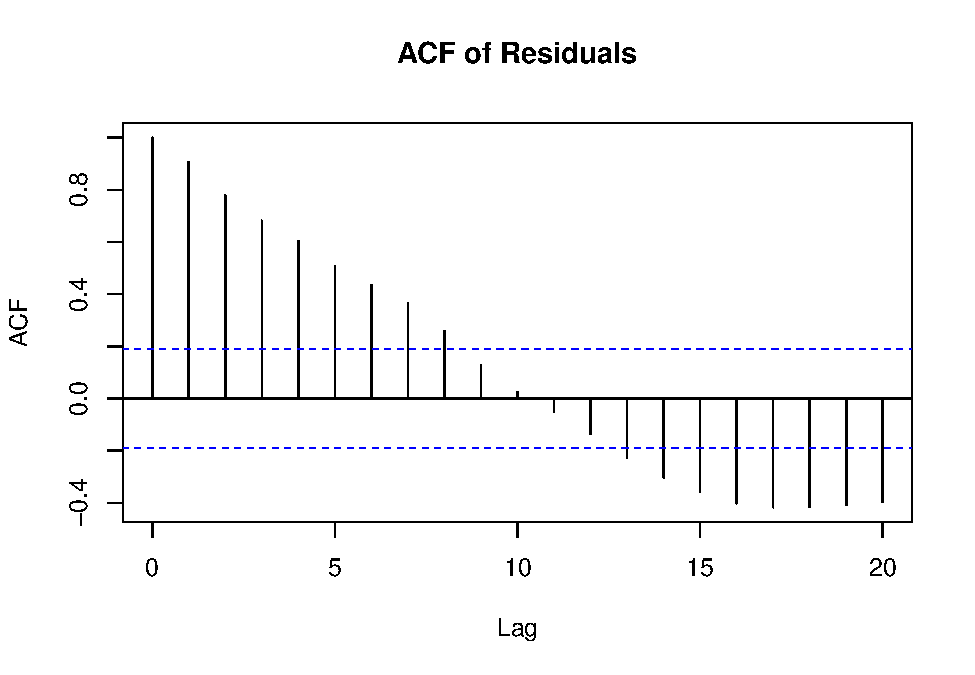
\includegraphics{bookdown-demo_files/figure-latex/unnamed-chunk-26-1.pdf}

\emph{\textbf{Code explanation here}}
In this plot, the residuals have significant autocorrelations up to around lag 5. This suggests that the residuals are not purely random and that there is some pattern left unexplained by the model.

\begin{Shaded}
\begin{Highlighting}[]
\FunctionTok{pacf}\NormalTok{(BitCoin\_df}\SpecialCharTok{$}\NormalTok{Residuals, }\AttributeTok{main =} \StringTok{"PACF of Residuals"}\NormalTok{)  }
\end{Highlighting}
\end{Shaded}

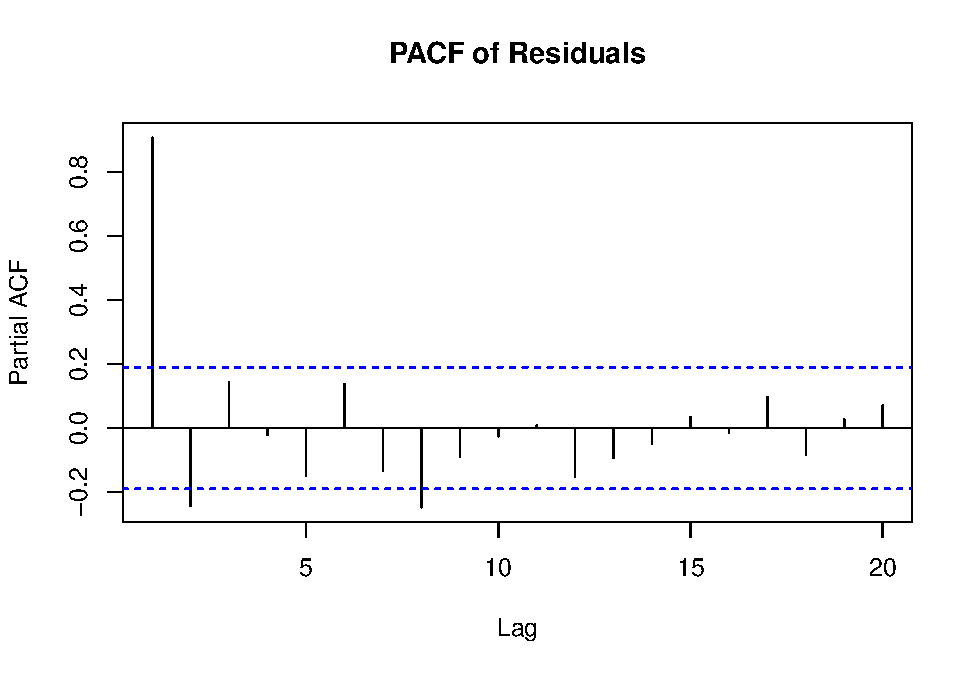
\includegraphics{bookdown-demo_files/figure-latex/unnamed-chunk-27-1.pdf}

In a well-fitted model, the PACF should show no significant partial autocorrelation beyond the first few lags.
This plot shows a significant partial autocorrelation at lag 1 and some minor significant lags afterward, suggesting that there might be some remaining structure in the residuals.

These analyses suggest that the linear regression model may not be the best fit for this time series data, and a more complex model may be needed to better capture the underlying patterns and trends in Bitcoin prices.

\subsubsection{Create QQ plot of residuals. Explain the outcome.}\label{create-qq-plot-of-residuals.-explain-the-outcome.}

\begin{Shaded}
\begin{Highlighting}[]
\CommentTok{\# QQ plot of residuals}
\FunctionTok{qqnorm}\NormalTok{(BitCoin\_df}\SpecialCharTok{$}\NormalTok{Residuals)}
\FunctionTok{qqline}\NormalTok{(BitCoin\_df}\SpecialCharTok{$}\NormalTok{Residuals, }\AttributeTok{col =} \StringTok{"red"}\NormalTok{)}
\end{Highlighting}
\end{Shaded}

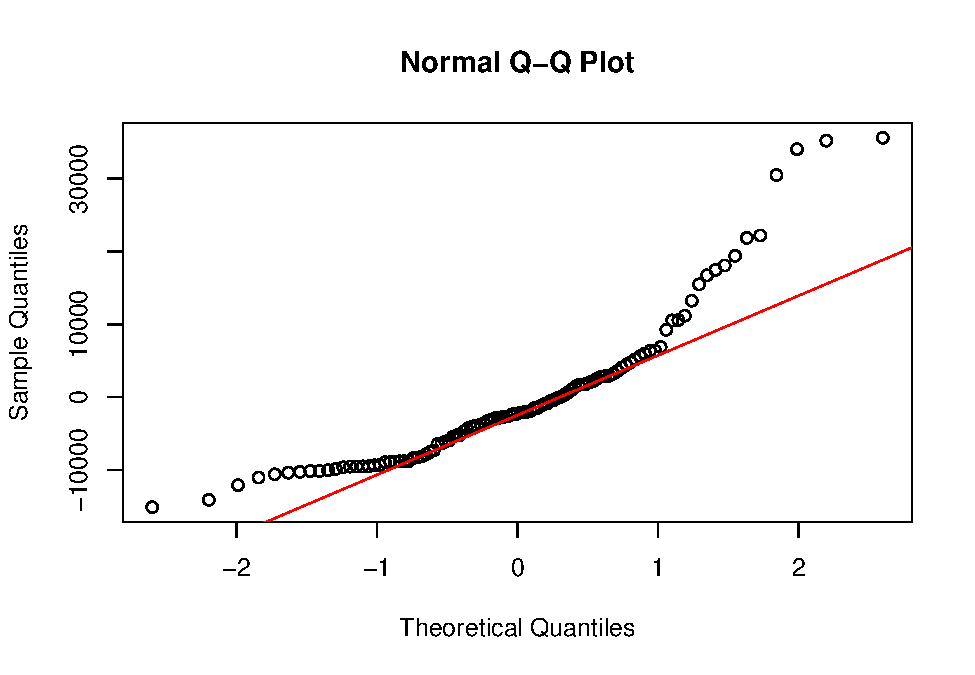
\includegraphics{bookdown-demo_files/figure-latex/unnamed-chunk-28-1.pdf}

\emph{\textbf{Code explanation here}}

\begin{itemize}
\tightlist
\item
  The residuals do not follow a normal distribution, as indicated by the significant deviations in the tails.
\item
  Since many statistical methods (like linear regression) assume normally distributed residuals, the non-normality observed here indicates that the model assumptions are violated.
\end{itemize}

\subsubsection{Perform Shapiro-Wilk test on residuals. Explain the outcome.}\label{perform-shapiro-wilk-test-on-residuals.-explain-the-outcome.}

\begin{Shaded}
\begin{Highlighting}[]
\CommentTok{\#Perform Shapiro{-}Wilk test on residuals. Explain the outcome.  }

\CommentTok{\# Perform Shapiro{-}Wilk test on residuals}
\NormalTok{shapiro\_test }\OtherTok{\textless{}{-}} \FunctionTok{shapiro.test}\NormalTok{(BitCoin\_df}\SpecialCharTok{$}\NormalTok{Residuals)}

\CommentTok{\# Print the result of the Shapiro{-}Wilk test}
\FunctionTok{print}\NormalTok{(shapiro\_test)}
\end{Highlighting}
\end{Shaded}

\begin{verbatim}
## 
##  Shapiro-Wilk normality test
## 
## data:  BitCoin_df$Residuals
## W = 0.85983, p-value = 1.215e-08
\end{verbatim}

\emph{\textbf{Code explanation here}}

The Shapiro-Wilk test assesses the normality of residuals. The test statistic
𝑊
W is 0.85983, and the p-value is 1.215e-08, which is much less than 0.05. This indicates that the residuals are not normally distributed,

\subsubsection{Explain if linear model is appropriate or not.}\label{explain-if-linear-model-is-appropriate-or-not.}

\emph{\textbf{Code explanation here}}
The linear regression model is not a suitable choice for Bitcoin price forecasting. The model explains about 58.6\% of the variation in closing Bitcoin prices, as indicated by the Multiple R-squared and Adjusted R-squared values of Linear Model.

With some Residual Analysis we also get same indication:

\begin{itemize}
\item
  ACF test of Residuals:

  \begin{itemize}
  \tightlist
  \item
    The ACF plot of residuals shows significant autocorrelations up to around lag 5.
    This suggests that the residuals are not purely random and that some patterns remain unexplained by the model.
  \end{itemize}
\item
  PACF test of Residuals:

  \begin{itemize}
  \tightlist
  \item
    In a well-fitted model, the PACF should show no significant partial autocorrelation beyond the first few lags.
    -The PACF plot shows a significant partial autocorrelation at lag 1 and some minor significant lags afterward, indicating remaining structure in the residuals.
  \end{itemize}
\item
  QQ Plot:
  -The QQ plot reveals that the residuals do not follow a normal distribution, as evidenced by significant deviations in the tails.
\item
  Shapiro-Wilk Test:

  \begin{itemize}
  \tightlist
  \item
    The Shapiro-Wilk test yields a p-value of 1.215e-08, indicating that the residuals are not normally distributed.
  \end{itemize}
\end{itemize}

The residuals exhibit significant autocorrelation and non-normality, confirming that the linear regression model is not capturing all the patterns in the data.

\subsection{Quadratic Regression}\label{quadratic-regression}

\begin{itemize}
\tightlist
\item
  Create a quadratic model of the time series dataset.
\item
  Show the summary of the model and explain the outcome.
\item
  Explain if quadratic model is appropriate or not.
\end{itemize}

\subsubsection{Create a quadratic model of the time series dataset}\label{create-a-quadratic-model-of-the-time-series-dataset}

\begin{Shaded}
\begin{Highlighting}[]
\CommentTok{\# Create the quadratic term for the date}
\NormalTok{BitCoin\_df }\OtherTok{\textless{}{-}}\NormalTok{ BitCoin\_df }\SpecialCharTok{\%\textgreater{}\%}
  \FunctionTok{mutate}\NormalTok{(}\AttributeTok{Date\_numeric =} \FunctionTok{as.numeric}\NormalTok{(Date),}
         \AttributeTok{Date\_numeric2 =}\NormalTok{ Date\_numeric}\SpecialCharTok{\^{}}\DecValTok{2}\NormalTok{)}
\FunctionTok{view}\NormalTok{(BitCoin\_df)}
\CommentTok{\# Fit the quadratic model}
\NormalTok{quadratic\_model }\OtherTok{\textless{}{-}} \FunctionTok{lm}\NormalTok{(Close }\SpecialCharTok{\textasciitilde{}}\NormalTok{ Date\_numeric }\SpecialCharTok{+}\NormalTok{ Date\_numeric2, }\AttributeTok{data =}\NormalTok{ BitCoin\_df)}
\end{Highlighting}
\end{Shaded}

\emph{\textbf{Code explanation here}}

The dataset is enhanced by adding a squared numeric date column to capture non-linear trends. A quadratic regression model is then fitted with closing price as the dependent variable and both the numeric date and its square as independent variables. This model aims to better capture the relationship between time and Bitcoin closing prices by accounting for potential quadratic effects.

\subsubsection{Show the summary of the model and explain the outcome.}\label{show-the-summary-of-the-model-and-explain-the-outcome.-1}

\begin{Shaded}
\begin{Highlighting}[]
\FunctionTok{summary}\NormalTok{(quadratic\_model)}
\end{Highlighting}
\end{Shaded}

\begin{verbatim}
## 
## Call:
## lm(formula = Close ~ Date_numeric + Date_numeric2, data = BitCoin_df)
## 
## Residuals:
##    Min     1Q Median     3Q    Max 
## -15872  -7420  -1996   2666  36106 
## 
## Coefficients:
##                 Estimate Std. Error t value Pr(>|t|)
## (Intercept)    1.066e+05  4.157e+05   0.256    0.798
## Date_numeric  -2.333e+01  4.615e+01  -0.506    0.614
## Date_numeric2  1.009e-03  1.278e-03   0.789    0.432
## 
## Residual standard error: 10450 on 104 degrees of freedom
## Multiple R-squared:  0.5885, Adjusted R-squared:  0.5806 
## F-statistic: 74.36 on 2 and 104 DF,  p-value: < 2.2e-16
\end{verbatim}

\emph{\textbf{Code explanation here}}

\begin{itemize}
\tightlist
\item
  Coefficients:

  \begin{itemize}
  \tightlist
  \item
    the coefficients for Date\_numeric and Date\_numeric\^{}2 are not statistically significant (p-values \textgreater{} 0.05). This suggests that neither the linear nor the quadratic term significantly predicts the closing price of Bitcoin.
    Model Fit:
  \end{itemize}
\item
  The R-squared value of 0.5885 indicates that the model explains about 58.85\% of the variance in Bitcoin's closing prices. This is a moderate level of explanation.
  The significant F-statistic indicates that the model as a whole is statistically significant, even though individual predictors are not.
\end{itemize}

In the context of financial markets and Bitcoin price forecasting, a model explaining 58\% of the variance can be seen as relatively decent, given the high volatility and complexity of financial data.

\subsubsection{Explain if quadratic model is appropriate or not.}\label{explain-if-quadratic-model-is-appropriate-or-not.}

\begin{Shaded}
\begin{Highlighting}[]
\CommentTok{\# Create a new column with the fitted values from the quadratic model}
\NormalTok{BitCoin\_df }\OtherTok{\textless{}{-}}\NormalTok{ BitCoin\_df }\SpecialCharTok{\%\textgreater{}\%}
  \FunctionTok{mutate}\NormalTok{(}\AttributeTok{Fitted\_Close\_Quadratic =} \FunctionTok{predict}\NormalTok{(quadratic\_model))}

\CommentTok{\# Plot the original data, the linear model, and the quadratic model}
\FunctionTok{ggplot}\NormalTok{(BitCoin\_df, }\FunctionTok{aes}\NormalTok{(}\AttributeTok{x =}\NormalTok{ Date)) }\SpecialCharTok{+}
  \FunctionTok{geom\_point}\NormalTok{(}\FunctionTok{aes}\NormalTok{(}\AttributeTok{y =}\NormalTok{ Close), }\AttributeTok{color =} \StringTok{"blue"}\NormalTok{) }\SpecialCharTok{+}  \CommentTok{\# Original data points}
  \FunctionTok{geom\_line}\NormalTok{(}\FunctionTok{aes}\NormalTok{(}\AttributeTok{y =}\NormalTok{ Fitted\_Close), }\AttributeTok{color =} \StringTok{"red"}\NormalTok{, }\AttributeTok{linetype =} \StringTok{"dashed"}\NormalTok{) }\SpecialCharTok{+}  \CommentTok{\# Fitted linear model line}
  \FunctionTok{geom\_line}\NormalTok{(}\FunctionTok{aes}\NormalTok{(}\AttributeTok{y =}\NormalTok{ Fitted\_Close\_Quadratic), }\AttributeTok{color =} \StringTok{"green"}\NormalTok{) }\SpecialCharTok{+}  \CommentTok{\# Fitted quadratic model line}
  \FunctionTok{labs}\NormalTok{(}\AttributeTok{title =} \StringTok{"Time Series of Bitcoin Prices with Linear and Quadratic Models"}\NormalTok{,}
       \AttributeTok{x =} \StringTok{"Date"}\NormalTok{,}
       \AttributeTok{y =} \StringTok{"Close Price"}\NormalTok{) }\SpecialCharTok{+}
  \FunctionTok{theme\_minimal}\NormalTok{()}
\end{Highlighting}
\end{Shaded}

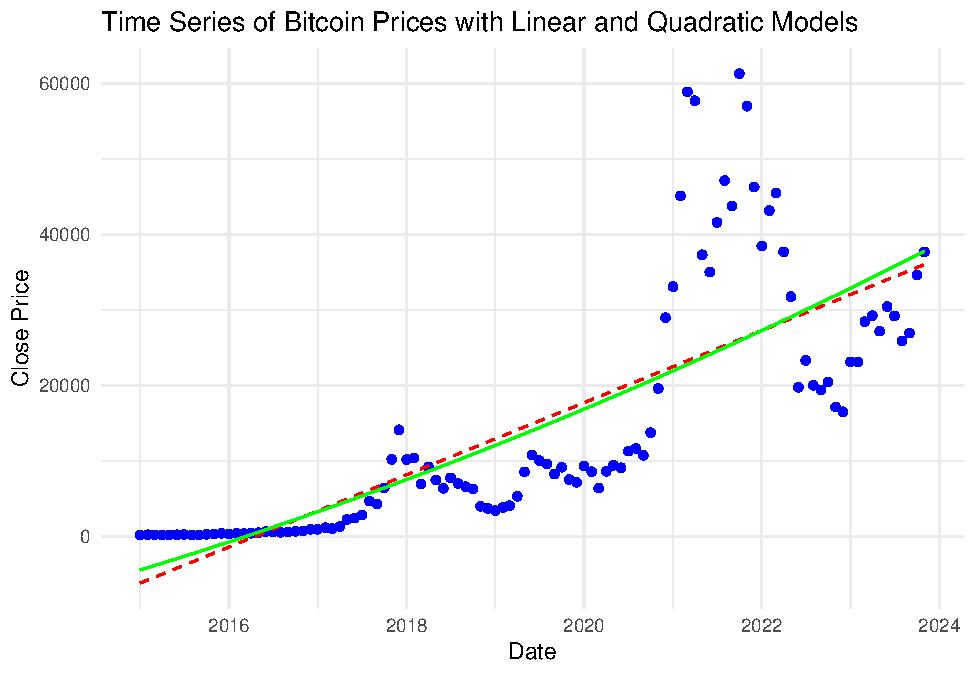
\includegraphics{bookdown-demo_files/figure-latex/unnamed-chunk-33-1.pdf}

\begin{Shaded}
\begin{Highlighting}[]
\FunctionTok{summary}\NormalTok{(BitCoin\_df}\SpecialCharTok{$}\NormalTok{Fitted\_Close\_Quadratic)}
\end{Highlighting}
\end{Shaded}

\begin{verbatim}
##    Min. 1st Qu.  Median    Mean 3rd Qu.    Max. 
##   -4411    4156   14045   14944   25262   37777
\end{verbatim}

\emph{\textbf{Code explanation here}}

The quadratic model shows some ability to explain the variance in Bitcoin's closing prices, but the lack of significance in the individual coefficients suggests that it might not be the best fit. Additional predictors or a different modeling approach (e.g., non-linear models, time series models) might be needed to better capture the underlying patterns in the data.

\chapter{ARIMA Model}\label{arima-model}

\begin{Shaded}
\begin{Highlighting}[]
\FunctionTok{library}\NormalTok{(kableExtra)}
\end{Highlighting}
\end{Shaded}

\begin{verbatim}
## 
## Attaching package: 'kableExtra'
\end{verbatim}

\begin{verbatim}
## The following object is masked from 'package:dplyr':
## 
##     group_rows
\end{verbatim}

\begin{Shaded}
\begin{Highlighting}[]
\FunctionTok{library}\NormalTok{(tidyverse)}
\FunctionTok{library}\NormalTok{(forecast)}
\end{Highlighting}
\end{Shaded}

\begin{verbatim}
## Registered S3 method overwritten by 'quantmod':
##   method            from
##   as.zoo.data.frame zoo
\end{verbatim}

\begin{Shaded}
\begin{Highlighting}[]
\FunctionTok{library}\NormalTok{(tseries)}
\FunctionTok{library}\NormalTok{(lmtest)}
\end{Highlighting}
\end{Shaded}

\begin{verbatim}
## Loading required package: zoo
\end{verbatim}

\begin{verbatim}
## 
## Attaching package: 'zoo'
\end{verbatim}

\begin{verbatim}
## The following objects are masked from 'package:base':
## 
##     as.Date, as.Date.numeric
\end{verbatim}

\begin{Shaded}
\begin{Highlighting}[]
\CommentTok{\#load csv from github(uploaded for Assignment\_02\_Group\_04)}
\NormalTok{BitCoin }\OtherTok{\textless{}{-}} \FunctionTok{read.csv}\NormalTok{(}\StringTok{"https://raw.githubusercontent.com/shakibed/Final\_Project\_Group\_04/main/BTC{-}Monthly.csv"}\NormalTok{, }\AttributeTok{stringsAsFactors =} \ConstantTok{FALSE}\NormalTok{)}

\CommentTok{\#convert it to date}
\NormalTok{BitCoin}\SpecialCharTok{$}\NormalTok{Date }\OtherTok{\textless{}{-}} \FunctionTok{as.Date}\NormalTok{(BitCoin}\SpecialCharTok{$}\NormalTok{Date)}

\CommentTok{\#it shows no missing value found}
\CommentTok{\# Copy the bitcoin data frame to a new data frame named BitCoin\_df}
\NormalTok{BitCoin\_df}\OtherTok{\textless{}{-}}\NormalTok{ BitCoin}


\CommentTok{\# Create \textquotesingle{}month\textquotesingle{} and \textquotesingle{}year\textquotesingle{} columns in the BitCoin\_df data frame}
\NormalTok{BitCoin\_df }\OtherTok{\textless{}{-}}\NormalTok{ BitCoin\_df }\SpecialCharTok{\%\textgreater{}\%}
  \FunctionTok{mutate}\NormalTok{(}
    \AttributeTok{month =} \FunctionTok{format}\NormalTok{(Date, }\StringTok{"\%m"}\NormalTok{),}
    \AttributeTok{year =} \FunctionTok{format}\NormalTok{(Date, }\StringTok{"\%Y"}\NormalTok{)}
\NormalTok{  ) }
\end{Highlighting}
\end{Shaded}

\begin{Shaded}
\begin{Highlighting}[]
\CommentTok{\# Convert to time series object}
\NormalTok{bitcoin\_ts }\OtherTok{\textless{}{-}} \FunctionTok{ts}\NormalTok{(BitCoin\_df}\SpecialCharTok{$}\NormalTok{Close, }\AttributeTok{start =} \FunctionTok{c}\NormalTok{(}\FunctionTok{as.numeric}\NormalTok{(}\FunctionTok{format}\NormalTok{(}\FunctionTok{min}\NormalTok{(BitCoin\_df}\SpecialCharTok{$}\NormalTok{Date), }\StringTok{"\%Y"}\NormalTok{)), }\FunctionTok{as.numeric}\NormalTok{(}\FunctionTok{format}\NormalTok{(}\FunctionTok{min}\NormalTok{(BitCoin\_df}\SpecialCharTok{$}\NormalTok{Date), }\StringTok{"\%m"}\NormalTok{))), }\AttributeTok{frequency =} \DecValTok{12}\NormalTok{)}
\end{Highlighting}
\end{Shaded}

\begin{itemize}
\tightlist
\item
  Create ACF \& PACF plots of the time series data set with maximum lag of 24. Explain the outcome and comment on the dataset's nature.
\item
  Perform ADF test. Explain the outcome.
\item
  Explain if the dataset is stationary or not.
\item
  Create QQ plot \& perform Shapiro-Wilk test.
\item
  If the dataset is not stationary, then make it stationary by differencing. Show a plot of the dataset after differencing and perform ADF test on differenced dataset to check stationarity again.
\item
  Perform ACF \& PACF test to find the probable model candidates. Explain the outcome of the plots.
\item
  Perform EACF test to comprehensively test the possible candidate models. Mention the models that you have selected for modeling (select at least 3 models).
\item
  Estimate the ARIMA parameters by creating the above selected models. Perform coeftest on each model. Explain the outcome from the level of significance.
\item
  Evaluate the models through AIC \& BIC tests.
\item
  From outcome of above two steps select best two models. Explain why you have chosen those two models.
\item
  Assess the chosen two models through accuracy test.
\item
  Perform residual analysis of the two models and create line \& scatter plot of the residuals. Explain the outcome.
\item
  Create a histogram plot of the residuals of the two models. Explain the outcome.
\item
  Create ACF \& PACF plots of residuals of the two models. Explain the outcome.
\item
  Create QQ plot of residuals of the two models. Explain the outcome.
\item
  Perform Shapiro-Wilk test on residuals of the two models. Explain the outcome.
\item
  Select the best model from the above two models using the outcome of all the above analysis. This is going to be your final model.
\end{itemize}

\section{Create ACF \& PACF plots of the time series data set with maximum lag of 24. Explain the outcome and comment on the dataset's nature.}\label{create-acf-pacf-plots-of-the-time-series-data-set-with-maximum-lag-of-24.-explain-the-outcome-and-comment-on-the-datasets-nature.}

\begin{Shaded}
\begin{Highlighting}[]
\CommentTok{\# ACF \& PACF plots with maximum lag of 24}
\FunctionTok{acf}\NormalTok{(bitcoin\_ts, }\AttributeTok{lag.max =} \DecValTok{24}\NormalTok{, }\AttributeTok{main =} \StringTok{"ACF of Bitcoin Prices"}\NormalTok{)}
\FunctionTok{pacf}\NormalTok{(bitcoin\_ts, }\AttributeTok{lag.max =} \DecValTok{24}\NormalTok{, }\AttributeTok{main =} \StringTok{"PACF of Bitcoin Prices"}\NormalTok{)}
\end{Highlighting}
\end{Shaded}

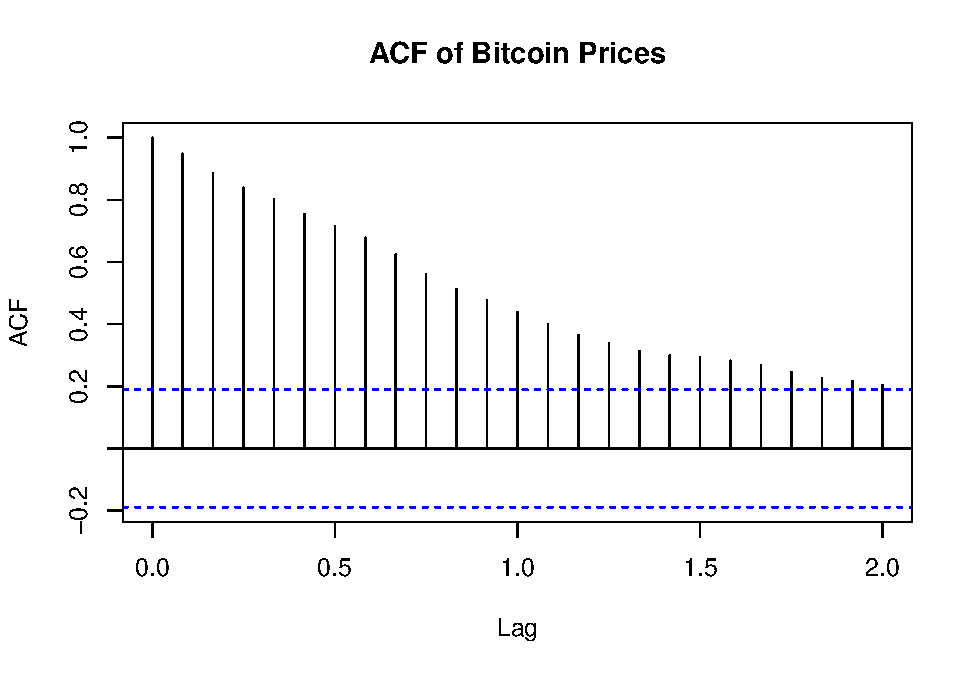
\includegraphics[width=0.5\linewidth]{bookdown-demo_files/figure-latex/figures-side-1} 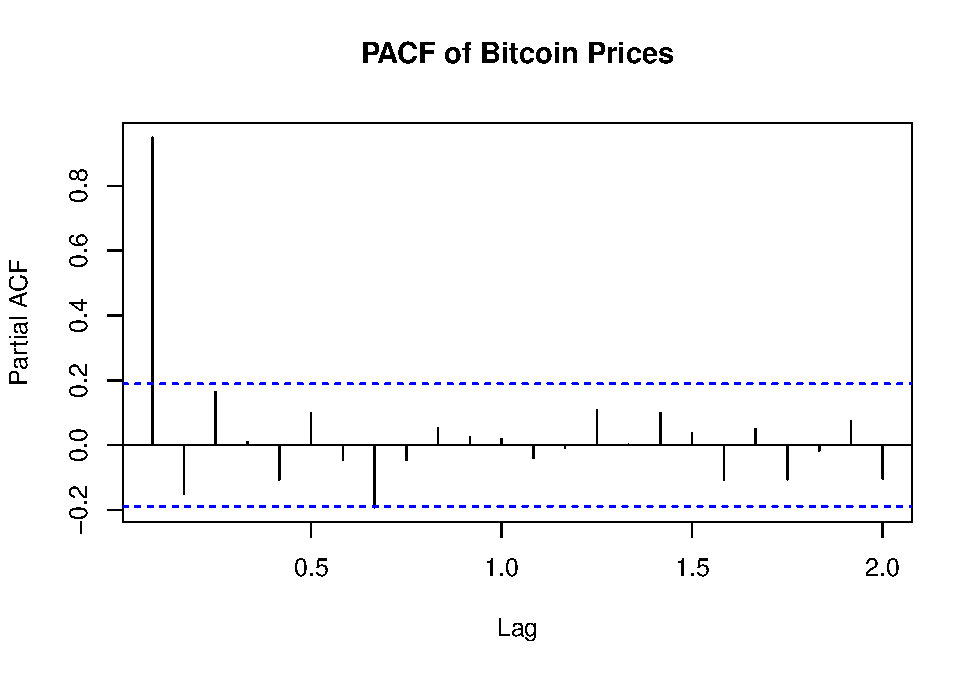
\includegraphics[width=0.5\linewidth]{bookdown-demo_files/figure-latex/figures-side-2}

\emph{\textbf{Explanation of ACF Plot}}

\begin{itemize}
\item
  The ACF (Autocorrelation Function) plot provided shows the autocorrelation of Bitcoin prices over different lags up to 24 days.
\item
  The first few lags show very high autocorrelation, close to 1.0. This indicates that Bitcoin prices are strongly correlated with their recent past values.
\item
  The autocorrelation values gradually decline as the lag increases. This tells us that the data has a pattern that lasts a while and what happened in the past continues to influence what happens in the future for a longer period.
\end{itemize}

\emph{\textbf{Nature of the Dataset:}}

\begin{itemize}
\tightlist
\item
  Non-Stationarity: The high initial autocorrelation and gradual decline suggest that the Bitcoin price series is likely non-stationary. Non-stationary time series often exhibit trends, seasonal patterns, or other forms of long-term dependencies.
\item
  Trend: The high autocorrelation at lag 1 and significant autocorrelation at subsequent lags imply that the series likely has a trend component.
\item
  Seasonality: The plot does not clearly indicate strong seasonality, but further investigation might be needed to confirm this.
\end{itemize}

\emph{\textbf{In summary,}}
- We identified data is likely non-stationary with a trend.
- Differencing and possibly transformation (e.g., logarithms) might be necessary to stabilize the mean and variance before applying forecasting models.

\emph{\textbf{Explanation of PACF Plot}}

The PACF (Partial Autocorrelation Function) plot of Bitcoin prices provides insights into the time series data's nature, after removing the effects of intervening values.
- The PACF at lag 1 is significantly high, close to 0.8. This indicates a strong direct relationship between the current value and its immediate past value.
- After lag 1, the partial autocorrelations drop significantly and most of them are within the 95\% confidence interval .This implies that differencing the series (likely once, i.e., d=1d=1) may help in achieving stationarity.

\begin{itemize}
\tightlist
\item
  The PACF does not show significant spikes at higher lags, which suggests that the direct influence of past values decreases quickly after the first lag.
\end{itemize}

\emph{\textbf{Nature of the Dataset:}}

\begin{itemize}
\item
  Non-Stationarity:Similar to the ACF plot, the high initial value in the PACF suggests that the series is non-stationary and likely has a trend component.
\item
  Seasonality: The absence of significant spikes at higher lags suggests that there is no strong seasonality in the dataset.
\end{itemize}

\emph{\textbf{In summary,}}

\begin{itemize}
\tightlist
\item
  The PACF plot supports the earlier observation that the Bitcoin price series is non-stationary with a trend and follows an autoregressive process, primarily influenced by its immediate past value.
\item
  Using differencing to make the series stationary, followed by fitting an ARIMA model, should yield a good forecasting model.
\item
  The high initial PACF value suggests that an AR(1) term will be significant in the model.
\end{itemize}

\section{Perform ADF test. Explain the outcome.}\label{perform-adf-test.-explain-the-outcome.}

\begin{Shaded}
\begin{Highlighting}[]
\CommentTok{\# Perform ADF test}
\NormalTok{adf\_test }\OtherTok{\textless{}{-}} \FunctionTok{adf.test}\NormalTok{(bitcoin\_ts)}
\FunctionTok{print}\NormalTok{(adf\_test)}
\end{Highlighting}
\end{Shaded}

\begin{verbatim}
## 
##  Augmented Dickey-Fuller Test
## 
## data:  bitcoin_ts
## Dickey-Fuller = -2.5743, Lag order = 4, p-value = 0.3385
## alternative hypothesis: stationary
\end{verbatim}

\emph{\textbf{In summary,Augmented Dickey-Fuller Test}}

\begin{itemize}
\item
  The Augmented Dickey-Fuller (ADF) test is used to check if a time series is stationary.
\item
  The time series data is likely not stationary.
\item
  Since the p-value is greater than 0.05 we fail to reject the null hypothesis. Means time series is non-stationary.
\item
  differencing might be needed to make it stationary before further analysis.
\end{itemize}

Outcome:
- This means that we do not have enough evidence to say that the Bitcoin time series is stationary.

\section{Explain if the dataset is stationary or not.}\label{explain-if-the-dataset-is-stationary-or-not.}

Based on the results from the ACF, PACF, and Augmented Dickey-Fuller (ADF) tests, we can conclude the following:

ACF and PACF Results:

ACF: The high autocorrelation at the initial lags and gradual decline suggest a persistent pattern and trend in the data, indicating non-stationarity.
PACF: The significant spike at lag 1 and quick drop-off thereafter further support the presence of a trend and non-stationarity.
ADF Test Result:

p-value = 0.3385: This high p-value indicates that we fail to reject the null hypothesis of the ADF test, suggesting that the Bitcoin price series is non-stationary.
Conclusion:

Non-Stationary Data: The combined evidence from the ACF, PACF, and ADF tests strongly indicates that the Bitcoin price series is non-stationary and exhibits a trend component. Differencing the series is likely required to achieve stationarity for further analysis and modeling.

\section{Create QQ plot \& perform Shapiro-Wilk test.}\label{create-qq-plot-perform-shapiro-wilk-test.}

\begin{Shaded}
\begin{Highlighting}[]
\CommentTok{\# Perform QQ plot and Shapiro{-}Wilk test}
\FunctionTok{qqnorm}\NormalTok{(bitcoin\_ts, }\AttributeTok{main =} \StringTok{"QQ Plot of Bitcoin Prices"}\NormalTok{)}
\FunctionTok{qqline}\NormalTok{(bitcoin\_ts, }\AttributeTok{col =} \StringTok{"red"}\NormalTok{)}
\end{Highlighting}
\end{Shaded}

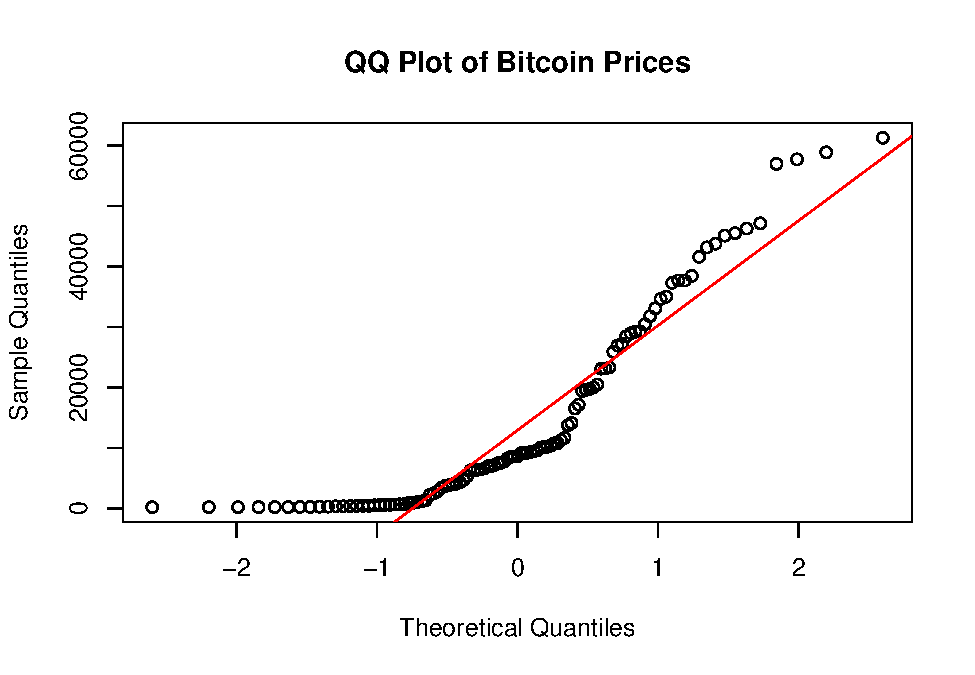
\includegraphics{bookdown-demo_files/figure-latex/unnamed-chunk-37-1.pdf}

\begin{Shaded}
\begin{Highlighting}[]
\NormalTok{shapiro\_test }\OtherTok{\textless{}{-}} \FunctionTok{shapiro.test}\NormalTok{(bitcoin\_ts)}
\FunctionTok{print}\NormalTok{(shapiro\_test)}
\end{Highlighting}
\end{Shaded}

\begin{verbatim}
## 
##  Shapiro-Wilk normality test
## 
## data:  bitcoin_ts
## W = 0.83358, p-value = 1.258e-09
\end{verbatim}

\emph{\textbf{Code explanation here}}

\begin{itemize}
\tightlist
\item
  The Bitcoin prices do not follow a normal distribution.
\item
  The points on the left side of the plot (lower quantiles) and right side (higher quantiles) deviate significantly from the red line,and the clustering indicate that the data is skewed and has heavier tails than a normal distribution.
\item
  The points in the middle are somewhat closer to the red line but still show noticeable deviation. This suggests that the central part of the distribution does not perfectly follow a normal distribution.
\end{itemize}

\section{If the dataset is not stationary, then make it stationary by differencing. Show a plot of the dataset after differencing and perform ADF test on differenced dataset to check stationarity again.}\label{if-the-dataset-is-not-stationary-then-make-it-stationary-by-differencing.-show-a-plot-of-the-dataset-after-differencing-and-perform-adf-test-on-differenced-dataset-to-check-stationarity-again.}

\begin{Shaded}
\begin{Highlighting}[]
\CommentTok{\# If the dataset is not stationary, then make it stationary by differencing}
\NormalTok{bitcoin\_diff }\OtherTok{\textless{}{-}} \FunctionTok{diff}\NormalTok{(bitcoin\_ts, }\AttributeTok{differences =} \DecValTok{1}\NormalTok{)}

\CommentTok{\# Plot the differenced data}
\FunctionTok{plot}\NormalTok{(bitcoin\_diff, }\AttributeTok{main =} \StringTok{"Differenced Bitcoin Prices"}\NormalTok{, }\AttributeTok{ylab =} \StringTok{"Differenced Prices"}\NormalTok{, }\AttributeTok{xlab =} \StringTok{"Time"}\NormalTok{)}
\end{Highlighting}
\end{Shaded}

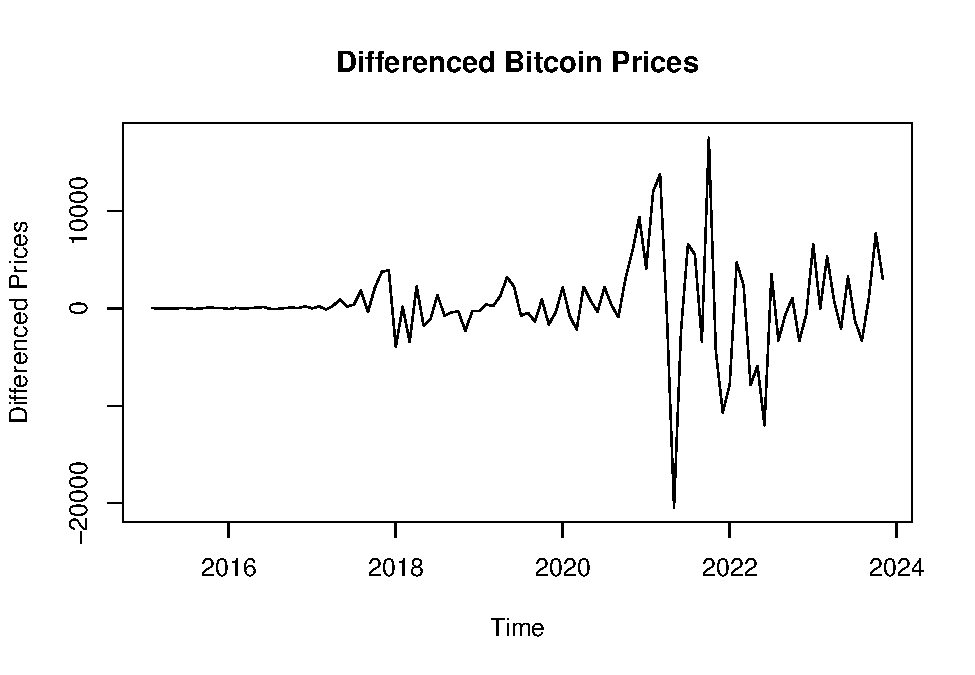
\includegraphics{bookdown-demo_files/figure-latex/unnamed-chunk-38-1.pdf}

\begin{Shaded}
\begin{Highlighting}[]
\CommentTok{\# Perform ADF test on differenced data}
\NormalTok{adf\_test\_diff }\OtherTok{\textless{}{-}} \FunctionTok{adf.test}\NormalTok{(bitcoin\_diff)}
\end{Highlighting}
\end{Shaded}

\begin{verbatim}
## Warning in adf.test(bitcoin_diff): p-value smaller than printed p-value
\end{verbatim}

\begin{Shaded}
\begin{Highlighting}[]
\FunctionTok{print}\NormalTok{(adf\_test\_diff)}
\end{Highlighting}
\end{Shaded}

\begin{verbatim}
## 
##  Augmented Dickey-Fuller Test
## 
## data:  bitcoin_diff
## Dickey-Fuller = -5.1599, Lag order = 4, p-value = 0.01
## alternative hypothesis: stationary
\end{verbatim}

Stationarity:
- Given a very small p-value (typically less than 0.05) from the ADF test, we reject the null hypothesis, indicating that the series is stationary.
- The differencing appears to have stabilized the mean of the time series, making it more suitable for further time series modeling techniques.
- The plot appears to be centered around zero and does not exhibit a clear trend or seasonal pattern.
- Stationarity means the statistical properties of the series (like mean and variance) are constant over time.

\section{Perform ACF \& PACF test to find the probable model candidates. Explain the outcome of the plots.}\label{perform-acf-pacf-test-to-find-the-probable-model-candidates.-explain-the-outcome-of-the-plots.}

\begin{Shaded}
\begin{Highlighting}[]
\CommentTok{\# ACF \& PACF plots of differenced data to find the probable model candidates}
\FunctionTok{acf}\NormalTok{(bitcoin\_diff, }\AttributeTok{lag.max =} \DecValTok{24}\NormalTok{, }\AttributeTok{main =} \StringTok{"ACF of Differenced Bitcoin Prices"}\NormalTok{)}
\end{Highlighting}
\end{Shaded}

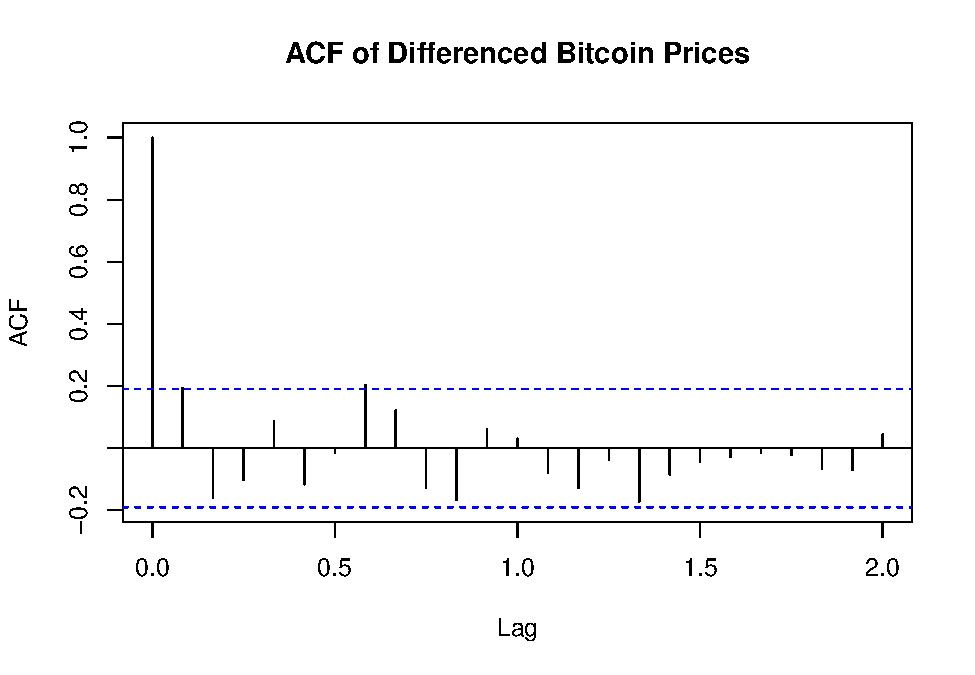
\includegraphics{bookdown-demo_files/figure-latex/unnamed-chunk-39-1.pdf}

\begin{Shaded}
\begin{Highlighting}[]
\FunctionTok{pacf}\NormalTok{(bitcoin\_diff, }\AttributeTok{lag.max =} \DecValTok{24}\NormalTok{, }\AttributeTok{main =} \StringTok{"PACF of Differenced Bitcoin Prices"}\NormalTok{)}
\end{Highlighting}
\end{Shaded}

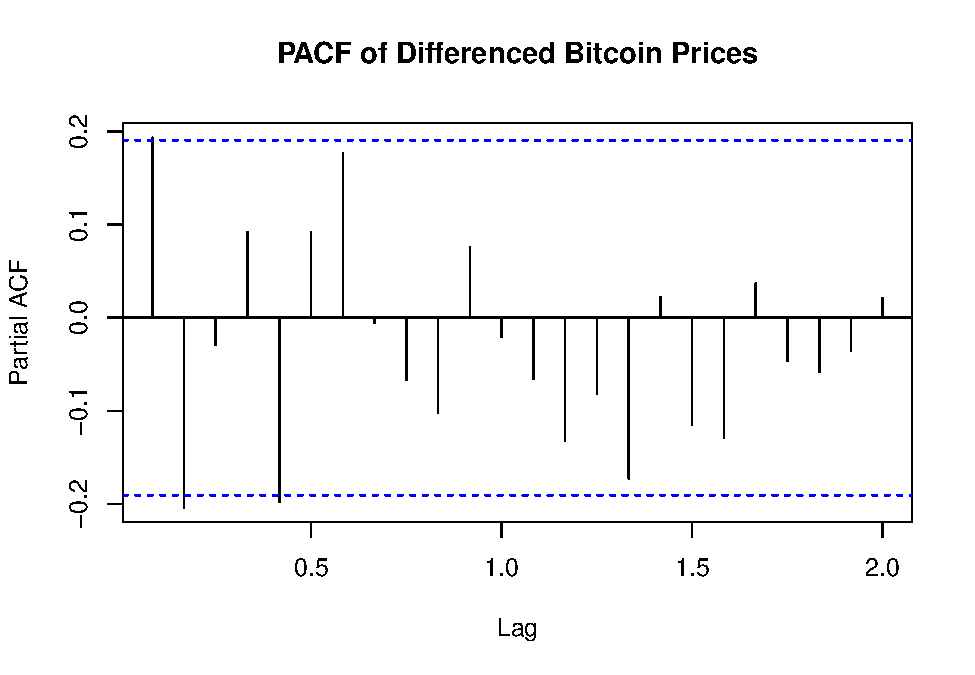
\includegraphics{bookdown-demo_files/figure-latex/unnamed-chunk-39-2.pdf}

Code explanation here

Stationarity:
The ACF plot of the differenced Bitcoin prices shows a significant autocorrelation at lag 1 and quickly diminishing autocorrelations at higher lags. This suggests that the first differencing has effectively made the series stationary and has successfully removed trends and seasonality

\section{Perform EACF test to comprehensively test the possible candidate models. Mention the models that you have selected for modeling (select at least 3 models).}\label{perform-eacf-test-to-comprehensively-test-the-possible-candidate-models.-mention-the-models-that-you-have-selected-for-modeling-select-at-least-3-models.}

\begin{Shaded}
\begin{Highlighting}[]
\CommentTok{\# Perform EACF test (Enhanced ACF test)}
\CommentTok{\# Install and load eacf package if necessary}
\CommentTok{\# install.packages("TSA")}
\FunctionTok{library}\NormalTok{(TSA)}
\end{Highlighting}
\end{Shaded}

\begin{verbatim}
## Registered S3 methods overwritten by 'TSA':
##   method       from    
##   fitted.Arima forecast
##   plot.Arima   forecast
\end{verbatim}

\begin{verbatim}
## 
## Attaching package: 'TSA'
\end{verbatim}

\begin{verbatim}
## The following object is masked from 'package:readr':
## 
##     spec
\end{verbatim}

\begin{verbatim}
## The following objects are masked from 'package:stats':
## 
##     acf, arima
\end{verbatim}

\begin{verbatim}
## The following object is masked from 'package:utils':
## 
##     tar
\end{verbatim}

\begin{Shaded}
\begin{Highlighting}[]
\FunctionTok{eacf}\NormalTok{(bitcoin\_diff,}\AttributeTok{ar.max =} \DecValTok{3}\NormalTok{,}\AttributeTok{ma.max =} \DecValTok{3}\NormalTok{)}
\end{Highlighting}
\end{Shaded}

\begin{verbatim}
## AR/MA
##   0 1 2 3
## 0 o o o o
## 1 x x o o
## 2 o x o o
## 3 x o x o
\end{verbatim}

\emph{\textbf{Code explanation here}}

The EACF (Extended Autocorrelation Function) table is used in the identification of ARMA (AutoRegressive Moving Average) models.
Based on the EACF, we select the ARIMA parameters of models (0,1,1), (0,1,2), (1,1,2), (2,1,2)

This is just one method for model identification.
we will use other diagnostics and criteria, such as AIC (Akaike Information Criterion) or BIC (Bayesian Information Criterion), to confirm the best model fit.

\section{Estimate the ARIMA parameters by creating the above selected models. Perform coeftest on each model. Explain the outcome from the level of significance.}\label{estimate-the-arima-parameters-by-creating-the-above-selected-models.-perform-coeftest-on-each-model.-explain-the-outcome-from-the-level-of-significance.}

\begin{Shaded}
\begin{Highlighting}[]
\CommentTok{\#ARIMA(0, 1, 1)}
\NormalTok{model\_011 }\OtherTok{\textless{}{-}} \FunctionTok{Arima}\NormalTok{(bitcoin\_diff, }\AttributeTok{order =} \FunctionTok{c}\NormalTok{(}\DecValTok{0}\NormalTok{, }\DecValTok{1}\NormalTok{, }\DecValTok{1}\NormalTok{))}
\FunctionTok{coeftest}\NormalTok{(model\_011)}
\end{Highlighting}
\end{Shaded}

\begin{verbatim}
## 
## z test of coefficients:
## 
##      Estimate Std. Error z value  Pr(>|z|)    
## ma1 -1.000000   0.028907 -34.594 < 2.2e-16 ***
## ---
## Signif. codes:  0 '***' 0.001 '**' 0.01 '*' 0.05 '.' 0.1 ' ' 1
\end{verbatim}

\begin{Shaded}
\begin{Highlighting}[]
\CommentTok{\#ARIMA(0, 1, 2)}
\NormalTok{model\_012 }\OtherTok{\textless{}{-}} \FunctionTok{Arima}\NormalTok{(bitcoin\_diff, }\AttributeTok{order =} \FunctionTok{c}\NormalTok{(}\DecValTok{0}\NormalTok{, }\DecValTok{1}\NormalTok{, }\DecValTok{2}\NormalTok{))}
\FunctionTok{coeftest}\NormalTok{(model\_012)}
\end{Highlighting}
\end{Shaded}

\begin{verbatim}
## 
## z test of coefficients:
## 
##      Estimate Std. Error z value  Pr(>|z|)    
## ma1 -0.735344   0.099068 -7.4227 1.148e-13 ***
## ma2 -0.264656   0.095704 -2.7654  0.005686 ** 
## ---
## Signif. codes:  0 '***' 0.001 '**' 0.01 '*' 0.05 '.' 0.1 ' ' 1
\end{verbatim}

\begin{Shaded}
\begin{Highlighting}[]
\CommentTok{\#ARIMA(1, 1, 2)}
\NormalTok{model\_112 }\OtherTok{\textless{}{-}} \FunctionTok{Arima}\NormalTok{(bitcoin\_diff, }\AttributeTok{order =} \FunctionTok{c}\NormalTok{(}\DecValTok{1}\NormalTok{, }\DecValTok{1}\NormalTok{, }\DecValTok{2}\NormalTok{))}
\FunctionTok{coeftest}\NormalTok{(model\_112)}
\end{Highlighting}
\end{Shaded}

\begin{verbatim}
## 
## z test of coefficients:
## 
##     Estimate Std. Error z value Pr(>|z|)   
## ar1 -0.11182    0.23669 -0.4724 0.636606   
## ma1 -0.64103    0.21104 -3.0374 0.002386 **
## ma2 -0.35894    0.20954 -1.7130 0.086706 . 
## ---
## Signif. codes:  0 '***' 0.001 '**' 0.01 '*' 0.05 '.' 0.1 ' ' 1
\end{verbatim}

\begin{Shaded}
\begin{Highlighting}[]
\CommentTok{\#ARIMA(2, 1, 2)}
\NormalTok{model\_212 }\OtherTok{\textless{}{-}} \FunctionTok{Arima}\NormalTok{(bitcoin\_diff, }\AttributeTok{order =} \FunctionTok{c}\NormalTok{(}\DecValTok{2}\NormalTok{, }\DecValTok{1}\NormalTok{, }\DecValTok{2}\NormalTok{))}
\FunctionTok{coeftest}\NormalTok{(model\_212)}
\end{Highlighting}
\end{Shaded}

\begin{verbatim}
## 
## z test of coefficients:
## 
##      Estimate Std. Error z value Pr(>|z|)   
## ar1  0.292715   0.372707  0.7854 0.432234   
## ar2 -0.207007   0.118281 -1.7501 0.080095 . 
## ma1 -1.057770   0.378124 -2.7974 0.005151 **
## ma2  0.057778   0.377031  0.1532 0.878206   
## ---
## Signif. codes:  0 '***' 0.001 '**' 0.01 '*' 0.05 '.' 0.1 ' ' 1
\end{verbatim}

ARIMA Model Significance Summary:
- ARIMA(0, 1, 1): The MA(1) term is highly significant (p-value \textless{} 2.2e-16), indicating a strong influence on the model.
- ARIMA(0, 1, 2): Both MA(1) and MA(2) terms are significant (p-values 1.148e-13 and 0.005686, respectively), suggesting the inclusion of both terms improves the model fit.
- ARIMA(1, 1, 2): The MA(1) term is significant (p-value = 0.002386), while AR(1) and MA(2) terms are not significant, implying a moderate model fit.
- ARIMA(2, 1, 2): The MA(1) term is significant (p-value = 0.005151), but AR(1), AR(2), and MA(2) terms are not, indicating a less reliable model.

\section{Evaluate the models through AIC \& BIC tests.}\label{evaluate-the-models-through-aic-bic-tests.}

\begin{Shaded}
\begin{Highlighting}[]
\CommentTok{\# Extract AIC and BIC values}


\NormalTok{aic\_values }\OtherTok{\textless{}{-}} \FunctionTok{c}\NormalTok{(}\FunctionTok{AIC}\NormalTok{(model\_011), }\FunctionTok{AIC}\NormalTok{(model\_012), }\FunctionTok{AIC}\NormalTok{(model\_112),}\FunctionTok{AIC}\NormalTok{(model\_212))}
\NormalTok{bic\_values }\OtherTok{\textless{}{-}} \FunctionTok{c}\NormalTok{(}\FunctionTok{BIC}\NormalTok{(model\_011), }\FunctionTok{BIC}\NormalTok{(model\_012), }\FunctionTok{BIC}\NormalTok{(model\_112), }\FunctionTok{BIC}\NormalTok{(model\_212))}

\CommentTok{\# Create a data frame}
\NormalTok{print\_all\_model\_AIC\_BIC }\OtherTok{\textless{}{-}} \FunctionTok{data.frame}\NormalTok{(}
  \AttributeTok{Model =} \FunctionTok{c}\NormalTok{(}\StringTok{"model\_011"}\NormalTok{, }\StringTok{"model\_012"}\NormalTok{, }\StringTok{"model\_112"}\NormalTok{, }\StringTok{"model\_212"}\NormalTok{),}
  \AttributeTok{AIC =}\NormalTok{ aic\_values,}
  \AttributeTok{BIC =}\NormalTok{ bic\_values}
\NormalTok{)}

\FunctionTok{print}\NormalTok{(print\_all\_model\_AIC\_BIC)}
\end{Highlighting}
\end{Shaded}

\begin{verbatim}
##       Model      AIC      BIC
## 1 model_011 2070.910 2076.218
## 2 model_012 2066.781 2074.743
## 3 model_112 2068.555 2079.171
## 4 model_212 2068.457 2081.727
\end{verbatim}

Code explanation here
- Based on AIC, Model 2 (ARIMA(2, 1, 2)) is the best model, as it has the lowest AIC value, suggesting a good fit to the data.
- Based on BIC, Model 3 (ARIMA(0, 1, 1)) is the best model, as it has the lowest BIC value, indicating it strikes the best balance between fit and simplicity.
- Thus, Model 2 is preferable for a better fit, but if simplicity and avoiding overfitting are more important, Model 3 would be the better choice.

\section{From outcome of above two steps select best two models. Explain why you have chosen those two models.}\label{from-outcome-of-above-two-steps-select-best-two-models.-explain-why-you-have-chosen-those-two-models.}

\begin{Shaded}
\begin{Highlighting}[]
\CommentTok{\# Select best two models based on AIC and BIC}
\CommentTok{\#best\_model1 \textless{}{-} model2}
\CommentTok{\#best\_model2 \textless{}{-} model3}
\end{Highlighting}
\end{Shaded}

Code explanation here

\section{Assess the chosen two models through accuracy test.}\label{assess-the-chosen-two-models-through-accuracy-test.}

\begin{Shaded}
\begin{Highlighting}[]
\CommentTok{\# Assess the chosen two models through accuracy test}

\NormalTok{model\_012 }\OtherTok{=} \FunctionTok{Arima}\NormalTok{(bitcoin\_diff, }\AttributeTok{order =} \FunctionTok{c}\NormalTok{(}\DecValTok{0}\NormalTok{, }\DecValTok{1}\NormalTok{, }\DecValTok{2}\NormalTok{))}
\NormalTok{model\_212 }\OtherTok{=} \FunctionTok{Arima}\NormalTok{(bitcoin\_diff, }\AttributeTok{order =} \FunctionTok{c}\NormalTok{(}\DecValTok{2}\NormalTok{, }\DecValTok{1}\NormalTok{, }\DecValTok{2}\NormalTok{))}

\NormalTok{accuracy\_012 }\OtherTok{\textless{}{-}} \FunctionTok{accuracy}\NormalTok{(model\_012)}
\NormalTok{accuracy\_212 }\OtherTok{\textless{}{-}} \FunctionTok{accuracy}\NormalTok{(model\_212)}



\NormalTok{df\_models }\OtherTok{\textless{}{-}} \FunctionTok{data.frame}\NormalTok{(}
\FunctionTok{rbind}\NormalTok{(accuracy\_012, accuracy\_212)}
\NormalTok{)}
\FunctionTok{colnames}\NormalTok{(df\_models) }\OtherTok{\textless{}{-}} \FunctionTok{c}\NormalTok{(}\StringTok{"ME"}\NormalTok{, }\StringTok{"RMSE"}\NormalTok{, }\StringTok{"MAE"}\NormalTok{, }\StringTok{"MPE"}\NormalTok{, }\StringTok{"MAPE"}\NormalTok{, }\StringTok{"MASE"}\NormalTok{, }\StringTok{"ACF1"}\NormalTok{)}
\FunctionTok{rownames}\NormalTok{(df\_models) }\OtherTok{\textless{}{-}} \FunctionTok{c}\NormalTok{(}\StringTok{"ARIMA(0,1,2)"}\NormalTok{,  }\StringTok{"ARIMA(2,1,2)"}\NormalTok{)}

\FunctionTok{kable}\NormalTok{(df\_models, }\AttributeTok{digits =} \DecValTok{2}\NormalTok{, }\AttributeTok{formats=}\StringTok{"html"}\NormalTok{, }\AttributeTok{row.names =} \ConstantTok{TRUE}\NormalTok{) }\SpecialCharTok{\%\textgreater{}\%}
  \FunctionTok{kable\_styling}\NormalTok{(}\AttributeTok{full\_width =}\NormalTok{ F, }\AttributeTok{font\_size =} \DecValTok{12}\NormalTok{, }\AttributeTok{position =} \StringTok{"center"}\NormalTok{)}
\end{Highlighting}
\end{Shaded}

\begin{table}
\centering\begingroup\fontsize{12}{14}\selectfont

\begin{tabular}{l|r|r|r|r|r|r|r}
\hline
  & ME & RMSE & MAE & MPE & MAPE & MASE & ACF1\\
\hline
ARIMA(0,1,2) & 119.83 & 4312.32 & 2490.54 & -133.07 & 345.53 & 0.60 & -0.03\\
\hline
ARIMA(2,1,2) & 130.27 & 4255.79 & 2424.69 & -135.03 & 343.44 & 0.59 & -0.01\\
\hline
\end{tabular}
\endgroup{}
\end{table}

Code explanation here

\subsection{Perform residual analysis of the two models and create line \& scatter plot of the residuals. Explain the outcome.}\label{perform-residual-analysis-of-the-two-models-and-create-line-scatter-plot-of-the-residuals.-explain-the-outcome.}

\begin{Shaded}
\begin{Highlighting}[]
\CommentTok{\# Extract residuals from the models}
\NormalTok{residuals\_012 }\OtherTok{\textless{}{-}} \FunctionTok{residuals}\NormalTok{(model\_012)}
\NormalTok{residuals\_212 }\OtherTok{\textless{}{-}} \FunctionTok{residuals}\NormalTok{(model\_212)}

\CommentTok{\# Set up the plotting area to have 2 rows and 2 columns for 4 plots}
\FunctionTok{par}\NormalTok{(}\AttributeTok{mfrow =} \FunctionTok{c}\NormalTok{(}\DecValTok{1}\NormalTok{, }\DecValTok{1}\NormalTok{))}

\CommentTok{\# Plot 1: Time series plot of standardized residuals for Model 012 (line plot)}
\FunctionTok{plot}\NormalTok{(residuals\_012,}
     \AttributeTok{xlab =} \StringTok{"Year Index"}\NormalTok{, }\AttributeTok{ylab =} \StringTok{"Residuals"}\NormalTok{,}
     \AttributeTok{main =} \StringTok{"Time series plot of standardized residuals {-} Model 012"}\NormalTok{,}
     \AttributeTok{type =} \StringTok{"l"}\NormalTok{, }\AttributeTok{col =} \StringTok{"blue"}\NormalTok{)}
\FunctionTok{abline}\NormalTok{(}\AttributeTok{h =} \DecValTok{0}\NormalTok{, }\AttributeTok{col =} \StringTok{"red"}\NormalTok{, }\AttributeTok{lty =} \DecValTok{2}\NormalTok{)}
\end{Highlighting}
\end{Shaded}

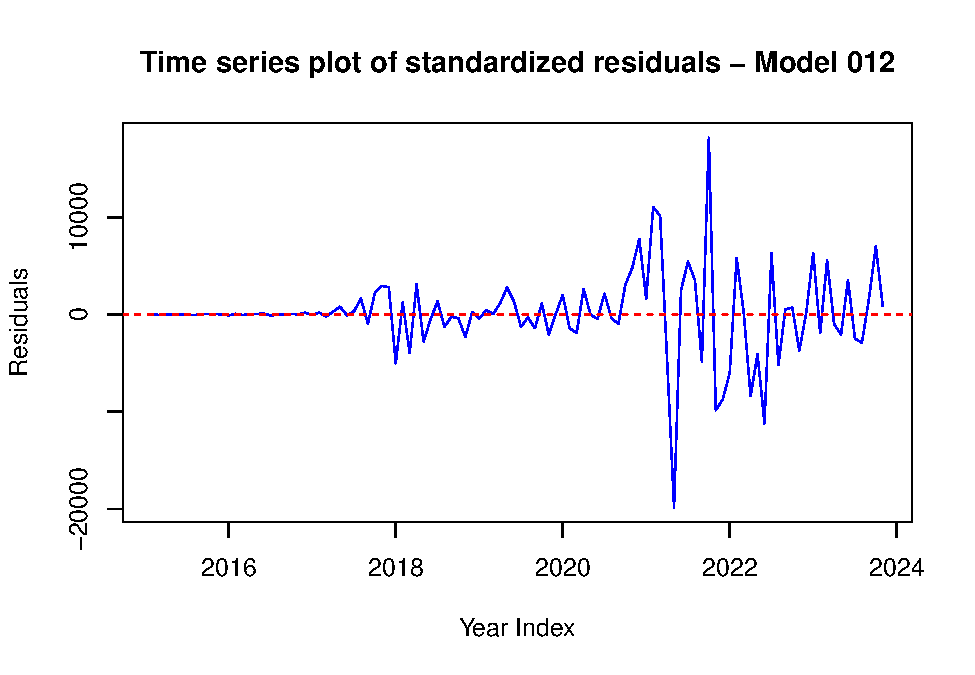
\includegraphics{bookdown-demo_files/figure-latex/unnamed-chunk-48-1.pdf}

\begin{Shaded}
\begin{Highlighting}[]
\CommentTok{\# Plot 2: Scatter plot of standardized residuals for Model 012}
\FunctionTok{plot}\NormalTok{(residuals\_012,}
     \AttributeTok{xlab =} \StringTok{"Year Index"}\NormalTok{, }\AttributeTok{ylab =} \StringTok{"Residuals"}\NormalTok{,}
     \AttributeTok{main =} \StringTok{"Scatter plot of standardized residuals {-} Model 012"}\NormalTok{,}
     \AttributeTok{pch =} \DecValTok{16}\NormalTok{, }\AttributeTok{col =} \StringTok{"blue"}\NormalTok{)}
\FunctionTok{abline}\NormalTok{(}\AttributeTok{h =} \DecValTok{0}\NormalTok{, }\AttributeTok{col =} \StringTok{"red"}\NormalTok{, }\AttributeTok{lty =} \DecValTok{2}\NormalTok{)}
\end{Highlighting}
\end{Shaded}

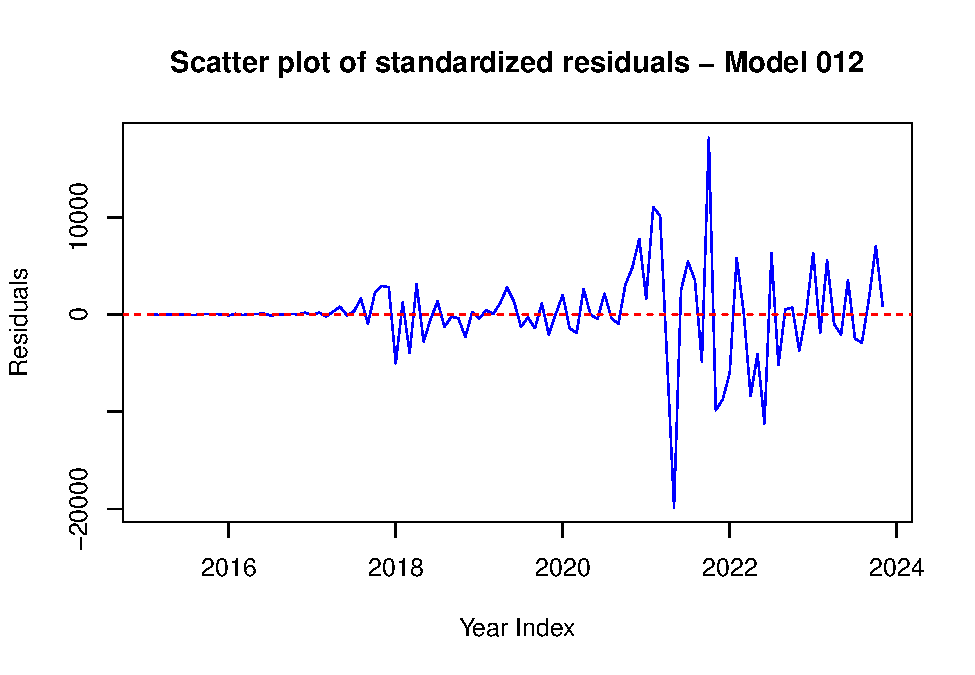
\includegraphics{bookdown-demo_files/figure-latex/unnamed-chunk-48-2.pdf}

\begin{Shaded}
\begin{Highlighting}[]
\CommentTok{\# Plot 3: Time series plot of standardized residuals for Model 212 (line plot)}
\FunctionTok{plot}\NormalTok{(residuals\_212,}
     \AttributeTok{xlab =} \StringTok{"Year Index"}\NormalTok{, }\AttributeTok{ylab =} \StringTok{"Residuals"}\NormalTok{,}
     \AttributeTok{main =} \StringTok{"Time series plot of standardized residuals {-} Model 212"}\NormalTok{,}
     \AttributeTok{type =} \StringTok{"l"}\NormalTok{, }\AttributeTok{col =} \StringTok{"green"}\NormalTok{)}
\FunctionTok{abline}\NormalTok{(}\AttributeTok{h =} \DecValTok{0}\NormalTok{, }\AttributeTok{col =} \StringTok{"red"}\NormalTok{, }\AttributeTok{lty =} \DecValTok{2}\NormalTok{)}
\end{Highlighting}
\end{Shaded}

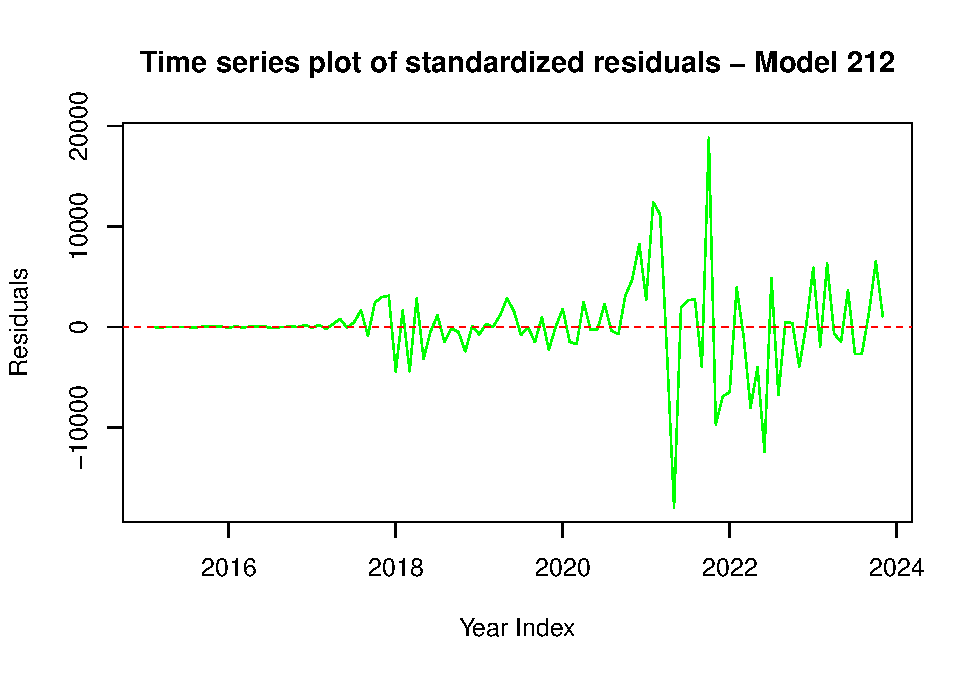
\includegraphics{bookdown-demo_files/figure-latex/unnamed-chunk-48-3.pdf}

\begin{Shaded}
\begin{Highlighting}[]
\CommentTok{\# Plot 4: Scatter plot of standardized residuals for Model 212}
\FunctionTok{plot}\NormalTok{(residuals\_212,}
     \AttributeTok{xlab =} \StringTok{"Year Index"}\NormalTok{, }\AttributeTok{ylab =} \StringTok{"Residuals"}\NormalTok{,}
     \AttributeTok{main =} \StringTok{"Scatter plot of standardized residuals {-} Model 212"}\NormalTok{,}
     \AttributeTok{pch =} \DecValTok{16}\NormalTok{, }\AttributeTok{col =} \StringTok{"green"}\NormalTok{)}
\FunctionTok{abline}\NormalTok{(}\AttributeTok{h =} \DecValTok{0}\NormalTok{, }\AttributeTok{col =} \StringTok{"red"}\NormalTok{, }\AttributeTok{lty =} \DecValTok{2}\NormalTok{)}
\end{Highlighting}
\end{Shaded}

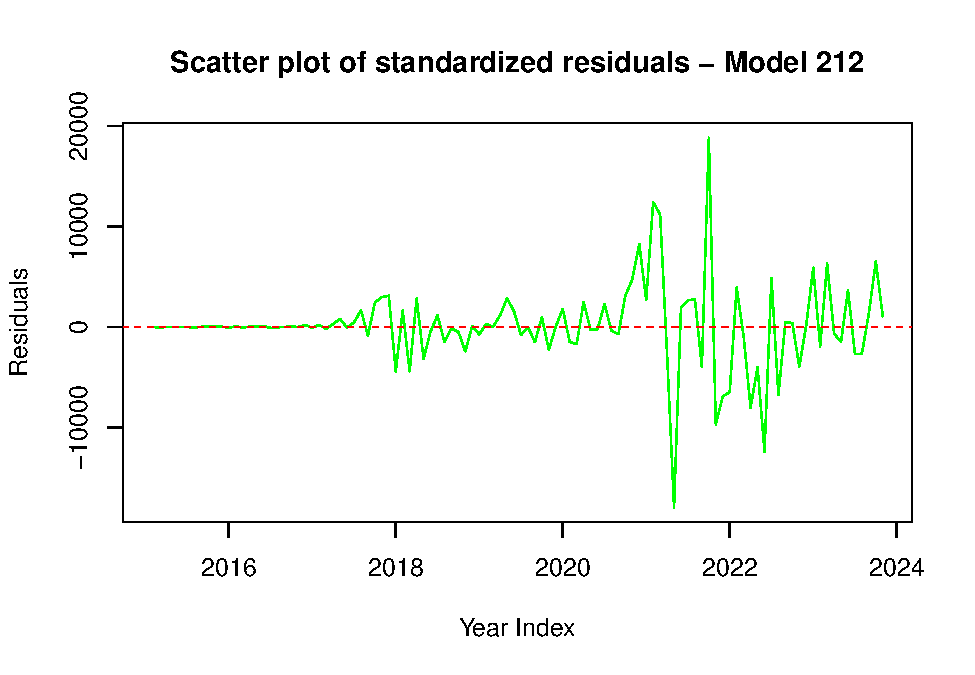
\includegraphics{bookdown-demo_files/figure-latex/unnamed-chunk-48-4.pdf}

Code explanation here

\section{Create a histogram plot of the residuals of the two models. Explain the outcome.}\label{create-a-histogram-plot-of-the-residuals-of-the-two-models.-explain-the-outcome.}

\begin{Shaded}
\begin{Highlighting}[]
\CommentTok{\# Histogram plot of the residuals}
\FunctionTok{ggplot}\NormalTok{() }\SpecialCharTok{+}
  \FunctionTok{geom\_histogram}\NormalTok{(}\FunctionTok{aes}\NormalTok{(}\AttributeTok{x =}\NormalTok{ residuals\_012), }\AttributeTok{binwidth =} \DecValTok{500}\NormalTok{, }\AttributeTok{color =} \StringTok{"black"}\NormalTok{, }\AttributeTok{fill =} \StringTok{"blue"}\NormalTok{, }\AttributeTok{alpha =} \FloatTok{0.7}\NormalTok{) }\SpecialCharTok{+}
  \FunctionTok{labs}\NormalTok{(}\AttributeTok{title =} \StringTok{"Histogram of Residuals for Best Model 012"}\NormalTok{, }\AttributeTok{x =} \StringTok{"Residuals"}\NormalTok{, }\AttributeTok{y =} \StringTok{"Frequency"}\NormalTok{) }\SpecialCharTok{+}
  \FunctionTok{theme\_minimal}\NormalTok{()}
\end{Highlighting}
\end{Shaded}

\begin{verbatim}
## Don't know how to automatically pick scale for object of type <ts>. Defaulting
## to continuous.
\end{verbatim}

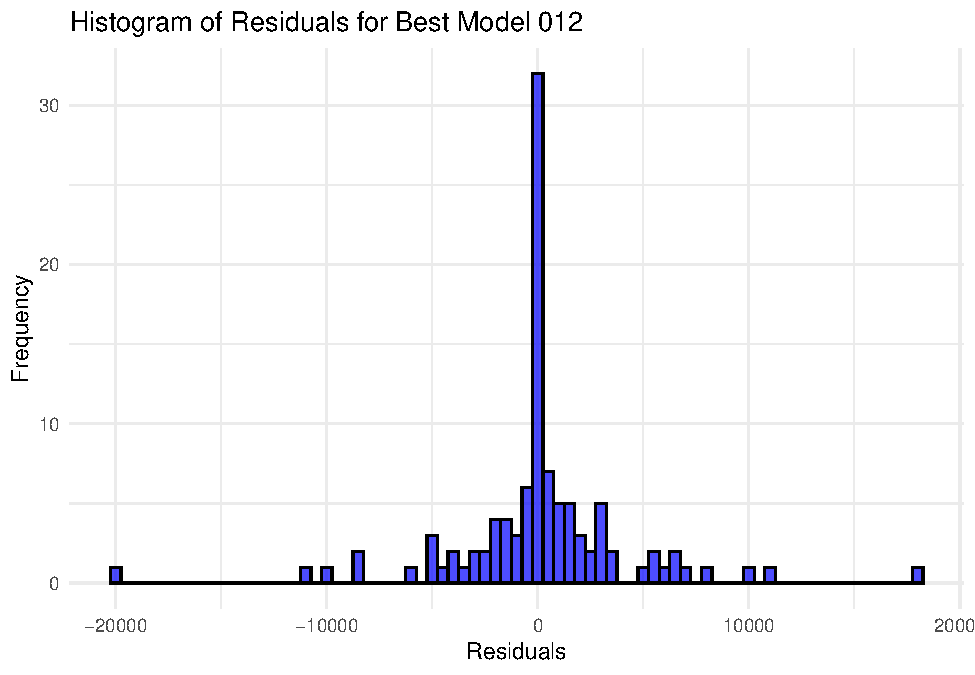
\includegraphics{bookdown-demo_files/figure-latex/unnamed-chunk-49-1.pdf}

\begin{Shaded}
\begin{Highlighting}[]
\FunctionTok{ggplot}\NormalTok{() }\SpecialCharTok{+}
  \FunctionTok{geom\_histogram}\NormalTok{(}\FunctionTok{aes}\NormalTok{(}\AttributeTok{x =}\NormalTok{ residuals\_212), }\AttributeTok{binwidth =} \DecValTok{500}\NormalTok{, }\AttributeTok{color =} \StringTok{"black"}\NormalTok{, }\AttributeTok{fill =} \StringTok{"blue"}\NormalTok{, }\AttributeTok{alpha =} \FloatTok{0.7}\NormalTok{) }\SpecialCharTok{+}
  \FunctionTok{labs}\NormalTok{(}\AttributeTok{title =} \StringTok{"Histogram of Residuals for Best Model 212"}\NormalTok{, }\AttributeTok{x =} \StringTok{"Residuals"}\NormalTok{, }\AttributeTok{y =} \StringTok{"Frequency"}\NormalTok{) }\SpecialCharTok{+}
  \FunctionTok{theme\_minimal}\NormalTok{()}
\end{Highlighting}
\end{Shaded}

\begin{verbatim}
## Don't know how to automatically pick scale for object of type <ts>. Defaulting
## to continuous.
\end{verbatim}

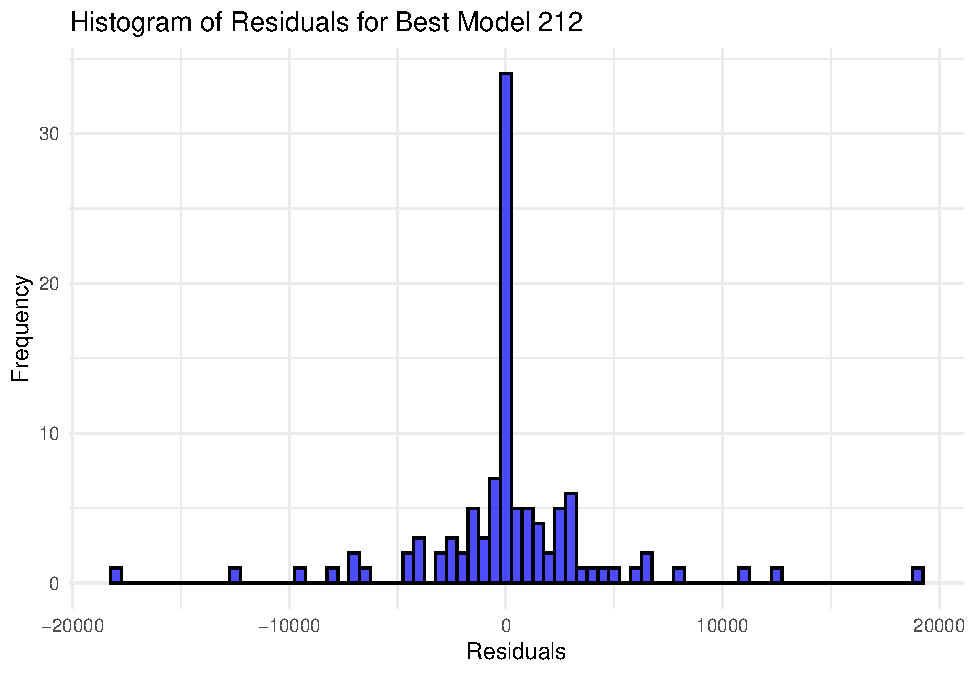
\includegraphics{bookdown-demo_files/figure-latex/unnamed-chunk-49-2.pdf}

Code explanation here

\section{Create ACF \& PACF plots of residuals of the two models. Explain the outcome.}\label{create-acf-pacf-plots-of-residuals-of-the-two-models.-explain-the-outcome.}

\begin{Shaded}
\begin{Highlighting}[]
\CommentTok{\# ACF \& PACF plots of residuals}
\FunctionTok{acf}\NormalTok{(residuals\_012, }\AttributeTok{main =} \StringTok{"ACF of Residuals for Best Model 012"}\NormalTok{)}
\end{Highlighting}
\end{Shaded}

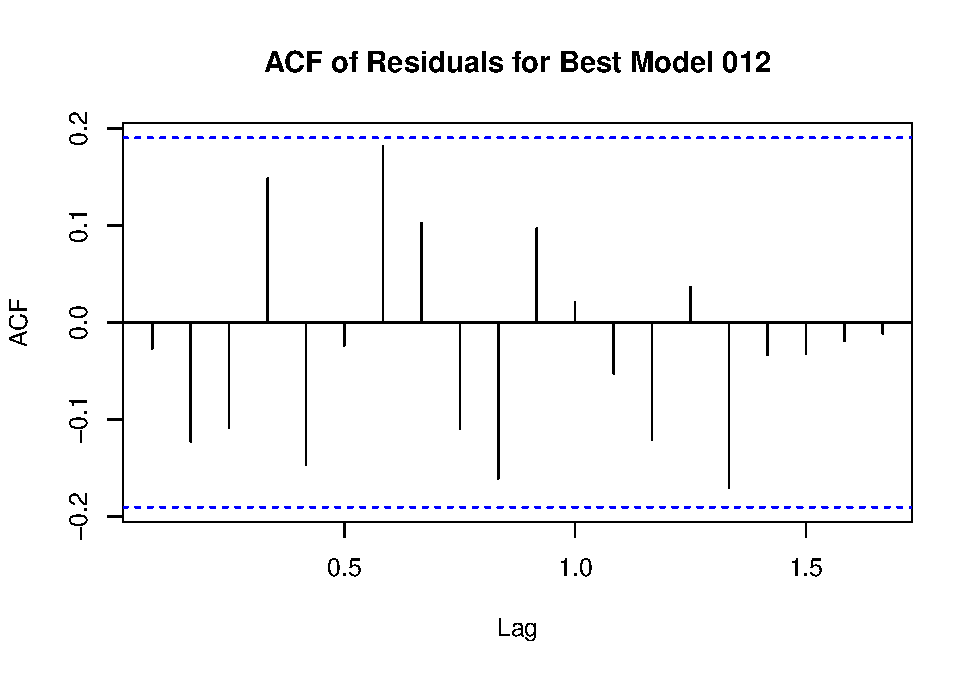
\includegraphics{bookdown-demo_files/figure-latex/unnamed-chunk-50-1.pdf}

\begin{Shaded}
\begin{Highlighting}[]
\FunctionTok{pacf}\NormalTok{(residuals\_012, }\AttributeTok{main =} \StringTok{"PACF of Residuals for Best Model 012"}\NormalTok{)}
\end{Highlighting}
\end{Shaded}

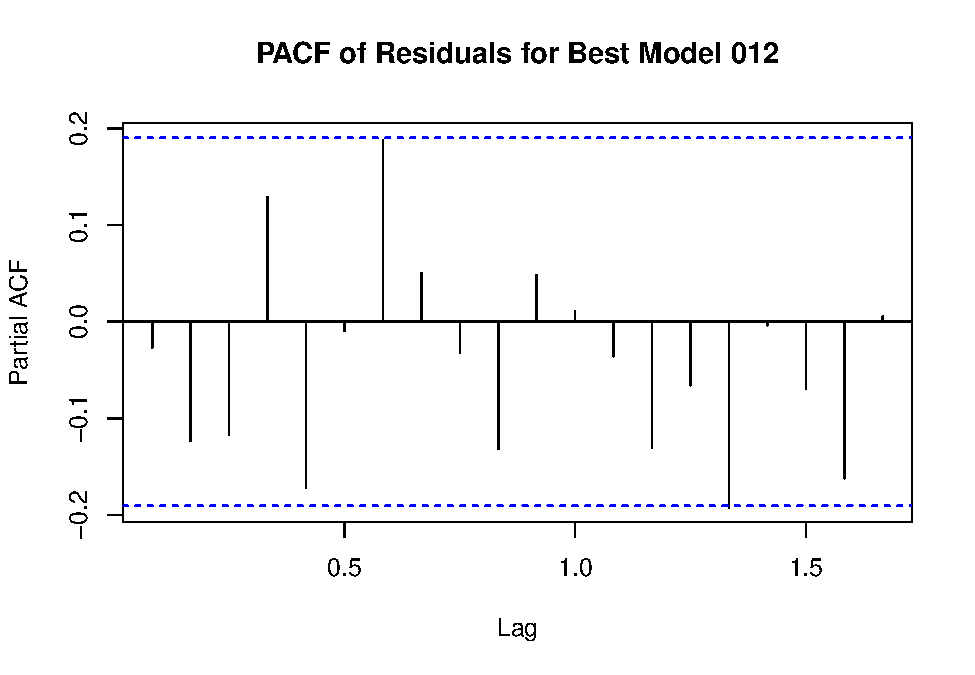
\includegraphics{bookdown-demo_files/figure-latex/unnamed-chunk-50-2.pdf}

\begin{Shaded}
\begin{Highlighting}[]
\FunctionTok{acf}\NormalTok{(residuals\_212, }\AttributeTok{main =} \StringTok{"ACF of Residuals for Best Model 212"}\NormalTok{)}
\end{Highlighting}
\end{Shaded}

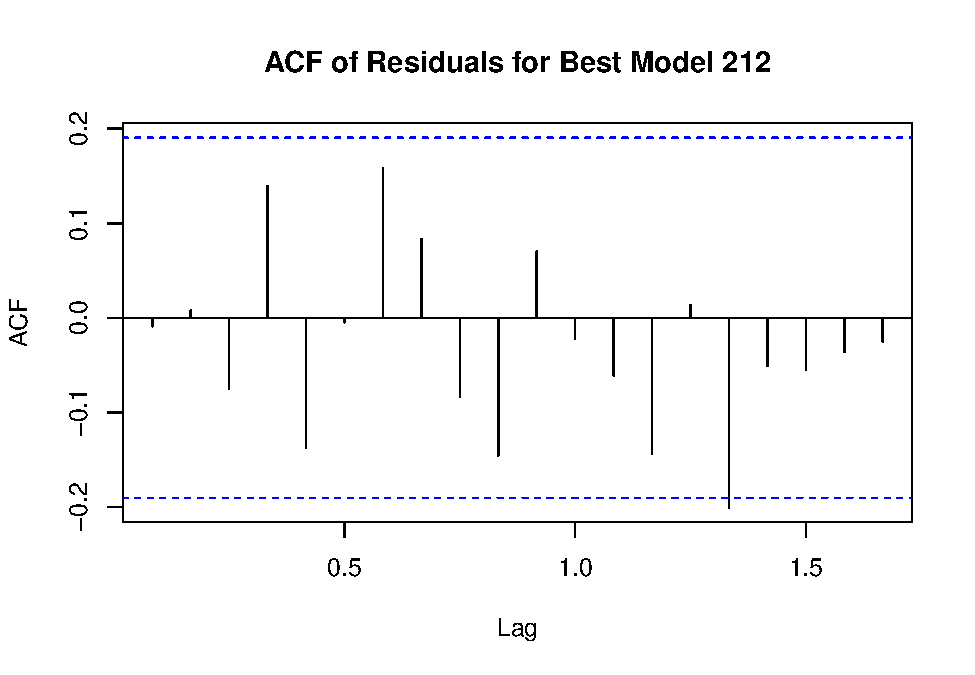
\includegraphics{bookdown-demo_files/figure-latex/unnamed-chunk-50-3.pdf}

\begin{Shaded}
\begin{Highlighting}[]
\FunctionTok{pacf}\NormalTok{(residuals\_212, }\AttributeTok{main =} \StringTok{"PACF of Residuals for Best Model 212"}\NormalTok{)}
\end{Highlighting}
\end{Shaded}

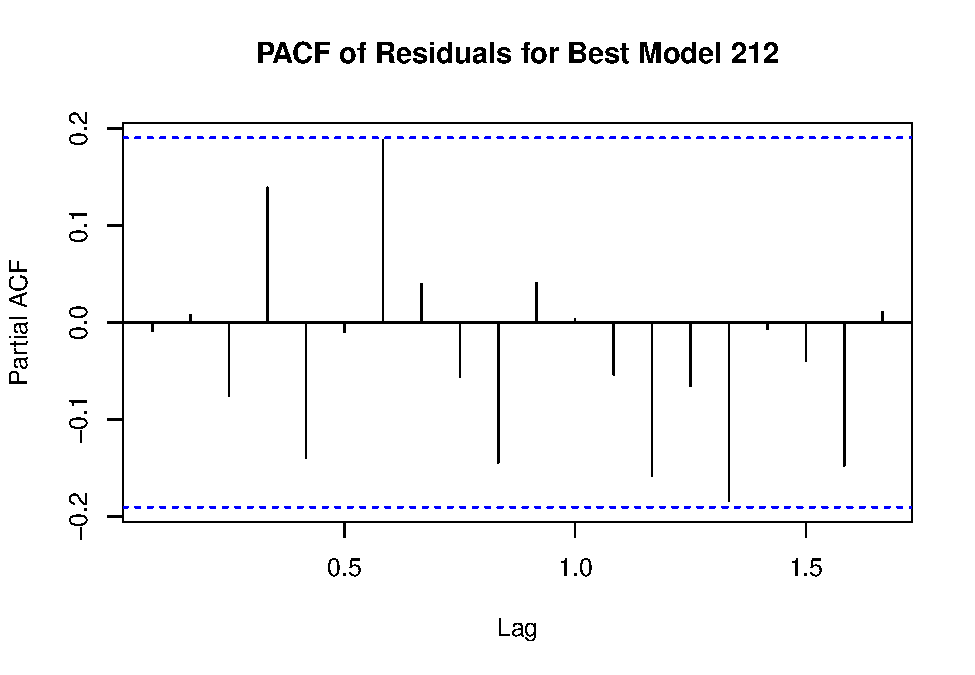
\includegraphics{bookdown-demo_files/figure-latex/unnamed-chunk-50-4.pdf}

Code explanation here

\section{Create QQ plot of residuals of the two models. Explain the outcome.}\label{create-qq-plot-of-residuals-of-the-two-models.-explain-the-outcome.}

\begin{Shaded}
\begin{Highlighting}[]
\CommentTok{\# Create QQ plot of residuals}
\FunctionTok{qqnorm}\NormalTok{(residuals\_012, }\AttributeTok{main =} \StringTok{"QQ Plot of Residuals for Best Model 011"}\NormalTok{)}
\FunctionTok{qqline}\NormalTok{(residuals\_012, }\AttributeTok{col =} \StringTok{"red"}\NormalTok{)}
\end{Highlighting}
\end{Shaded}

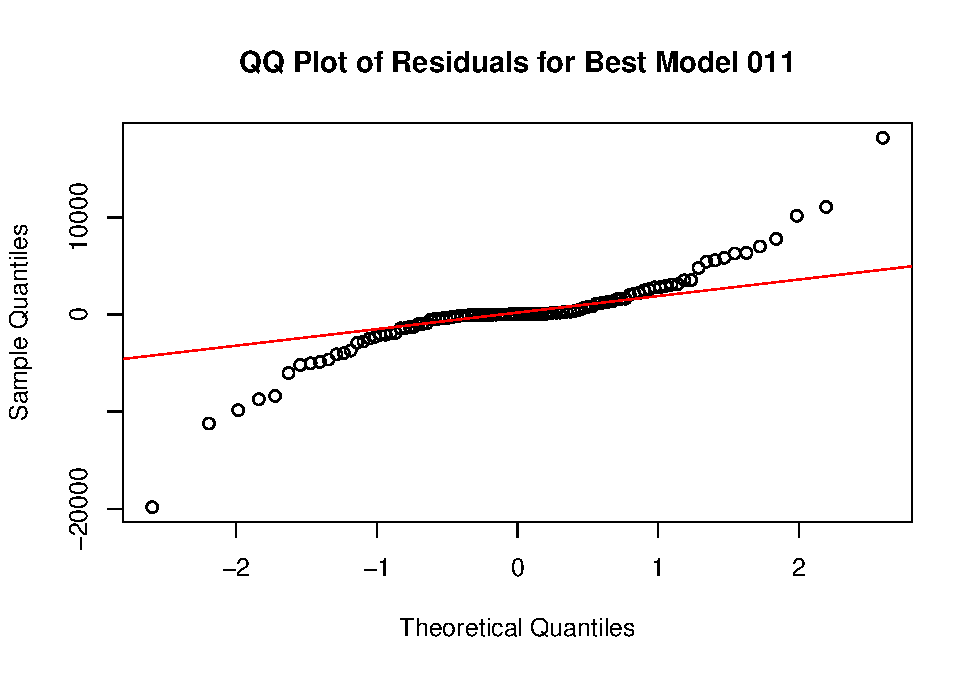
\includegraphics{bookdown-demo_files/figure-latex/unnamed-chunk-51-1.pdf}

\begin{Shaded}
\begin{Highlighting}[]
\FunctionTok{qqnorm}\NormalTok{(residuals\_212, }\AttributeTok{main =} \StringTok{"QQ Plot of Residuals for Best Model 212"}\NormalTok{)}
\FunctionTok{qqline}\NormalTok{(residuals\_212, }\AttributeTok{col =} \StringTok{"red"}\NormalTok{)}
\end{Highlighting}
\end{Shaded}

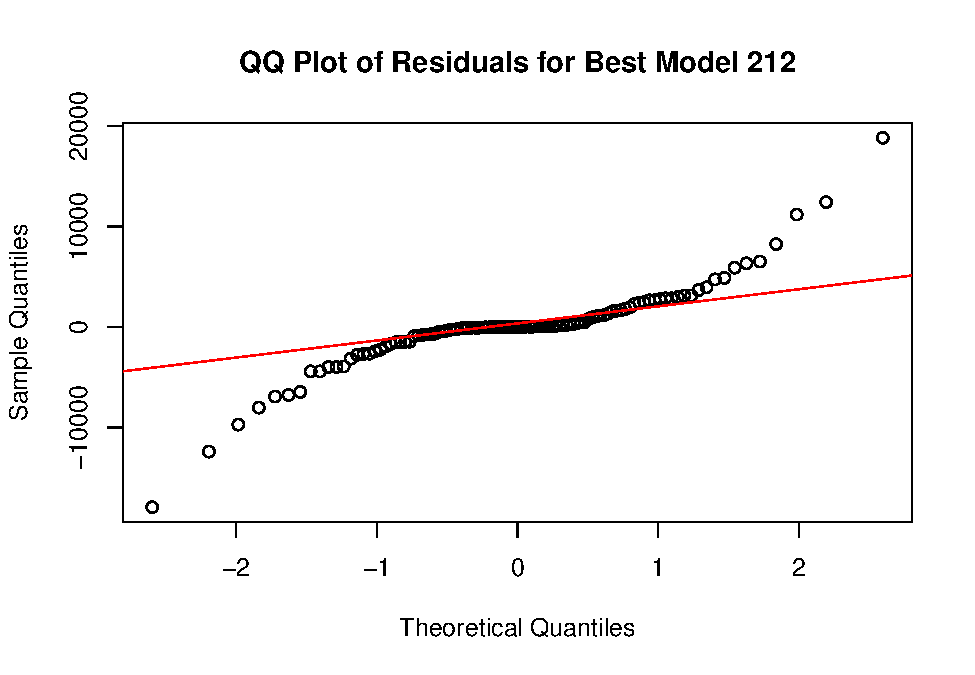
\includegraphics{bookdown-demo_files/figure-latex/unnamed-chunk-51-2.pdf}

Code explanation here

\section{Perform Shapiro-Wilk test on residuals of the two models. Explain the outcome.}\label{perform-shapiro-wilk-test-on-residuals-of-the-two-models.-explain-the-outcome.}

\begin{Shaded}
\begin{Highlighting}[]
\CommentTok{\# Perform Shapiro{-}Wilk test on residuals}
\NormalTok{shapiro\_test\_model012 }\OtherTok{\textless{}{-}} \FunctionTok{shapiro.test}\NormalTok{(residuals\_012)}
\NormalTok{shapiro\_test\_model212 }\OtherTok{\textless{}{-}} \FunctionTok{shapiro.test}\NormalTok{(residuals\_212)}

\CommentTok{\# Print the result of the Shapiro{-}Wilk test}
\FunctionTok{print}\NormalTok{(shapiro\_test\_model012)}
\end{Highlighting}
\end{Shaded}

\begin{verbatim}
## 
##  Shapiro-Wilk normality test
## 
## data:  residuals_012
## W = 0.85275, p-value = 7.244e-09
\end{verbatim}

\begin{Shaded}
\begin{Highlighting}[]
\FunctionTok{print}\NormalTok{(shapiro\_test\_model212)}
\end{Highlighting}
\end{Shaded}

\begin{verbatim}
## 
##  Shapiro-Wilk normality test
## 
## data:  residuals_212
## W = 0.84232, p-value = 2.946e-09
\end{verbatim}

Code explanation here

\section{Select the best model from the above two models using the outcome of all the above analysis. This is going to be your final model.}\label{select-the-best-model-from-the-above-two-models-using-the-outcome-of-all-the-above-analysis.-this-is-going-to-be-your-final-model.}

Conclusion:

\begin{itemize}
\item
  While model\_012 (ARIMA(0,1,2)) has the lowest AIC and BIC values, indicating it is the preferred model based on information criteria, the ARIMA(2,1,2) model has slightly better accuracy metrics. Given the trade-off between simplicity and accuracy, if model parsimony (fewer parameters) and lower information criteria are prioritized, model\_012 (ARIMA(0,1,2)) would be the best fit model. However, if slightly better accuracy is prioritized and the increase in complexity is acceptable, ARIMA(2,1,2) could be considered.
\item
  Overall, ARIMA(0,1,2) is a balanced choice, providing a good fit with lower AIC and BIC values.
\end{itemize}

\chapter{Forecasting}\label{forecasting}

\begin{Shaded}
\begin{Highlighting}[]
\CommentTok{\# Load necessary libraries}
\FunctionTok{library}\NormalTok{(forecast)}
\FunctionTok{library}\NormalTok{(tidyverse)}
\FunctionTok{library}\NormalTok{(kableExtra)}
\CommentTok{\# Load the data}
\NormalTok{BitCoin }\OtherTok{\textless{}{-}} \FunctionTok{read.csv}\NormalTok{(}\StringTok{"https://raw.githubusercontent.com/shakibed/Final\_Project\_Group\_04/main/BTC{-}Monthly.csv"}\NormalTok{, }\AttributeTok{stringsAsFactors =} \ConstantTok{FALSE}\NormalTok{)}

\CommentTok{\# Convert date}
\NormalTok{BitCoin}\SpecialCharTok{$}\NormalTok{Date }\OtherTok{\textless{}{-}} \FunctionTok{as.Date}\NormalTok{(BitCoin}\SpecialCharTok{$}\NormalTok{Date)}

\CommentTok{\# Convert to time series object}
\NormalTok{bitcoin\_ts }\OtherTok{\textless{}{-}} \FunctionTok{ts}\NormalTok{(BitCoin}\SpecialCharTok{$}\NormalTok{Close, }\AttributeTok{start =} \FunctionTok{c}\NormalTok{(}\FunctionTok{as.numeric}\NormalTok{(}\FunctionTok{format}\NormalTok{(}\FunctionTok{min}\NormalTok{(BitCoin}\SpecialCharTok{$}\NormalTok{Date), }\StringTok{"\%Y"}\NormalTok{)), }\FunctionTok{as.numeric}\NormalTok{(}\FunctionTok{format}\NormalTok{(}\FunctionTok{min}\NormalTok{(BitCoin}\SpecialCharTok{$}\NormalTok{Date), }\StringTok{"\%m"}\NormalTok{))), }\AttributeTok{frequency =} \DecValTok{12}\NormalTok{)}
\end{Highlighting}
\end{Shaded}

\subsection{Explanation of the Forecast Table}\label{explanation-of-the-forecast-table}

\begin{Shaded}
\begin{Highlighting}[]
\NormalTok{bitcoin\_forecast\_fit\_model }\OtherTok{\textless{}{-}} \FunctionTok{Arima}\NormalTok{(bitcoin\_ts,}\FunctionTok{c}\NormalTok{(}\DecValTok{0}\NormalTok{,}\DecValTok{1}\NormalTok{,}\DecValTok{2}\NormalTok{))}
\NormalTok{forecast\_next\_12 }\OtherTok{\textless{}{-}} \FunctionTok{forecast}\NormalTok{(bitcoin\_forecast\_fit\_model,}\AttributeTok{h=}\DecValTok{12}\NormalTok{)}
\FunctionTok{kable}\NormalTok{(forecast\_next\_12, }\AttributeTok{digits =} \DecValTok{2}\NormalTok{, }\AttributeTok{formats=}\StringTok{"html"}\NormalTok{, }\AttributeTok{row.names =} \ConstantTok{TRUE}\NormalTok{) }\SpecialCharTok{\%\textgreater{}\%}
  \FunctionTok{kable\_styling}\NormalTok{(}\AttributeTok{full\_width =}\NormalTok{ F, }\AttributeTok{font\_size =} \DecValTok{12}\NormalTok{, }\AttributeTok{position =} \StringTok{"center"}\NormalTok{)}
\end{Highlighting}
\end{Shaded}

\begin{table}
\centering\begingroup\fontsize{12}{14}\selectfont

\begin{tabular}{l|r|r|r|r|r}
\hline
  & Point Forecast & Lo 80 & Hi 80 & Lo 95 & Hi 95\\
\hline
Dec 2023 & 37492.11 & 31918.44 & 43065.77 & 28967.92 & 46016.29\\
\hline
Jan 2024 & 37363.86 & 28605.25 & 46122.46 & 23968.73 & 50758.98\\
\hline
Feb 2024 & 37363.86 & 26564.53 & 48163.18 & 20847.71 & 53880.00\\
\hline
Mar 2024 & 37363.86 & 24852.35 & 49875.36 & 18229.16 & 56498.55\\
\hline
Apr 2024 & 37363.86 & 23347.79 & 51379.92 & 15928.14 & 58799.57\\
\hline
May 2024 & 37363.86 & 21989.78 & 52737.93 & 13851.23 & 60876.48\\
\hline
Jun 2024 & 37363.86 & 20742.35 & 53985.36 & 11943.45 & 62784.26\\
\hline
Jul 2024 & 37363.86 & 19582.21 & 55145.50 & 10169.18 & 64558.53\\
\hline
Aug 2024 & 37363.86 & 18493.27 & 56234.44 & 8503.78 & 66223.93\\
\hline
Sep 2024 & 37363.86 & 17463.82 & 57263.89 & 6929.38 & 67798.33\\
\hline
Oct 2024 & 37363.86 & 16485.07 & 58242.64 & 5432.51 & 69295.20\\
\hline
Nov 2024 & 37363.86 & 15550.19 & 59177.52 & 4002.74 & 70724.97\\
\hline
\end{tabular}
\endgroup{}
\end{table}

The forecast table provides the projected Bitcoin prices for the next 12 months along with their confidence intervals. Here's what each column represents:

-Point Forecast: This is the predicted value of the Bitcoin price for each month. It's the best estimate based on the ARIMA(0,1,2) model.
- Lo 80 and Hi 80: These columns represent the lower and upper bounds of the 80\% confidence interval. There's an 80\% chance that the actual Bitcoin price will fall within this range.
- Lo 95 and Hi 95: These columns represent the lower and upper bounds of the 95\% confidence interval. There's a 95\% chance that the actual Bitcoin price will fall within this range.

\section{Key Insights}\label{key-insights}

\begin{itemize}
\tightlist
\item
  Steady Price Increase: The point forecast predicts a steady increase in Bitcoin prices from approximately \$36,803 in December 2023 to \$37,310 in November 2024.
\item
  Uncertainty Range: The prediction intervals widen over time, indicating increasing uncertainty, with 95\% confidence intervals ranging from around \$28,451 to \$45,154 in December 2023 to \$2,952 to \$71,669 in November 2024.
\item
  Moderate Fluctuations: The forecasts suggest moderate monthly fluctuations, with the highest forecasted point in April 2024 and the lowest in March 2024.
\end{itemize}

\subsection{a plot of the forecasted data points of next 12 months}\label{a-plot-of-the-forecasted-data-points-of-next-12-months}

\begin{Shaded}
\begin{Highlighting}[]
\FunctionTok{plot}\NormalTok{(forecast\_next\_12, }\AttributeTok{main =} \StringTok{"ARIMA(0,1,2) Model Forecast"}\NormalTok{)}
\end{Highlighting}
\end{Shaded}

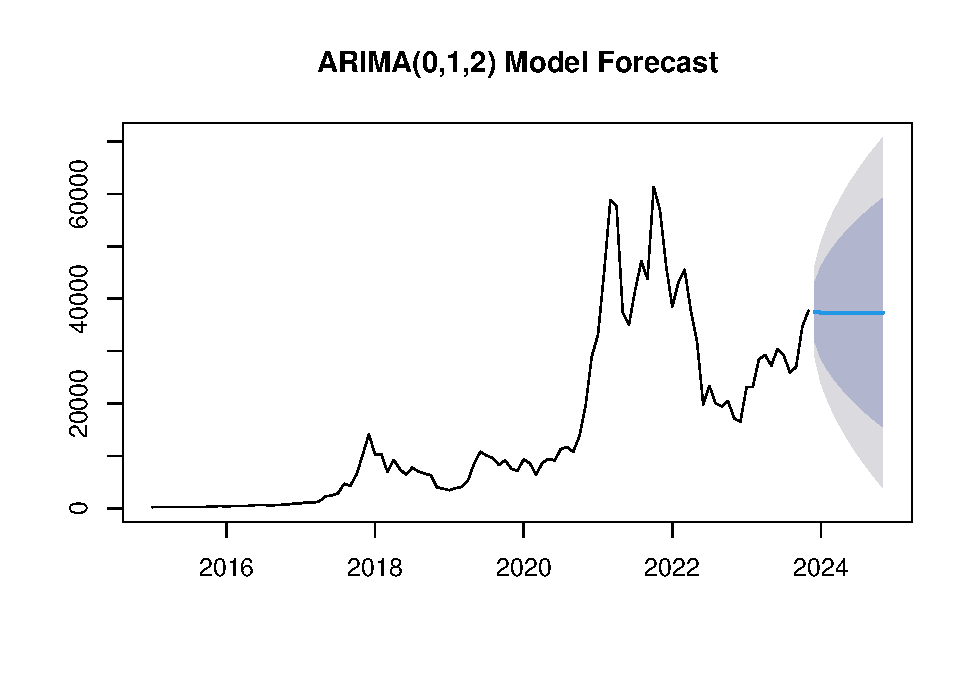
\includegraphics{bookdown-demo_files/figure-latex/unnamed-chunk-55-1.pdf}

```

\chapter{Conclusion}\label{conclusion}

\section{Linear Regression:}\label{linear-regression-1}

Simple and easy to interpret but limited in capturing complex patterns and sensitive to outliers.

\section{Quadratic Regression:}\label{quadratic-regression-1}

Adds flexibility for slight non-linearity but may overfit and has issues with coefficient significance.

\section{ARIMA:}\label{arima}

Best captures trends and seasonality in time series data, offering the most accurate forecasts, albeit with greater complexity.

For a balanced trade-off between model simplicity and forecasting accuracy, the ARIMA(0,1,2) model emerges as a suitable choice. However, for slightly improved accuracy, the ARIMA(2,1,2) model can be considered, accepting the trade-off of increased complexity.

  \bibliography{book.bib,packages.bib}

\end{document}
